\documentclass[spanish]{beamer}
%% \usetheme{Warsaw}
%% \usetheme{Madrid}

\usepackage[spanish]{babel}
\usetheme[beetle]{Boadilla}


 \useoutertheme{miniframes}
%% \useinnertheme{rounded}
%% \usecolortheme{}
\usepackage[utf8]{inputenc}
\usepackage{tikz}
\usepackage{wrapfig}
%% \usepackage{authblk}


%% \setbeameroption{show notes}


\usepackage{graphicx} 
\usepackage{algorithmic}
\usepackage{algorithm}
\newcommand{\formulasize}{\tiny}

\definecolor{rojo}{rgb}{0.7,0.1,0.1}
\definecolor{azul}{rgb}{0.1,0.1,0.7}
\definecolor{verde}{rgb}{0.1,0.4,0.1}

\newcommand{\rojo}[1]{\textcolor{rojo}{#1}}
\newcommand{\azul}[1]{\textcolor{azul}{#1}}
\newcommand{\verde}[1]{\textcolor{verde}{#1}}

%% \setcounter{secnumdepth}{5}

\newcommand{\Rojo}[1]{\textbf{\rojo{#1}}}
\newcommand{\Azul}[1]{\textbf{\azul{#1}}}
\newcommand{\Verde}[1]{\textbf{\verde{#1}}}

%%% Unified concepts commands

\newcommand{\opencl}{\emph{OpenCL}}

\newcommand{\pipeline}{\emph{pipeline}}
\newcommand{\Pipeline}{\emph{Pipeline}}

\newcommand{\wi}{\emph{work item}}
\newcommand{\wis}{\emph{work items}}
\newcommand{\wg}{\emph{work group}}
\newcommand{\wgs}{\emph{work groups}}

\newcommand{\Wi}{\emph{Work item}}
\newcommand{\Wis}{\emph{Work items}}
\newcommand{\Wg}{\emph{Work group}}
\newcommand{\Wgs}{\emph{Work groups}}

\newcommand{\bbox}{BBox}
\newcommand{\bboxes}{BBoxes}
\newcommand{\bvh}{BVH}
\newcommand{\bvhs}{BVHs}

\newcommand {\raytracer}{\emph{ray tracer}}
\newcommand {\raytracers}{\emph{ray tracers}}
\newcommand {\raytracing}{\emph{ray tracing}}
\newcommand {\Raytracer}{\emph{Ray tracer}}
\newcommand {\Raytracers}{\emph{Ray tracers}}
\newcommand {\Raytracing}{\emph{Ray tracing}}

%%% Style fix so institue doesnt appear on brackets (props to Claudio Fiandrino)
\setbeamertemplate{footline}{
  \leavevmode%
  \hbox{%
  \begin{beamercolorbox}[wd=.333333\paperwidth,ht=2.25ex,dp=1ex,center]{author in head/foot}%
    \usebeamerfont{author in head/foot}\insertshortauthor
  \end{beamercolorbox}%
  \begin{beamercolorbox}[wd=.333333\paperwidth,ht=2.25ex,dp=1ex,center]{title in head/foot}%
    \usebeamerfont{title in head/foot}\insertshorttitle
  \end{beamercolorbox}%
  \begin{beamercolorbox}[wd=.333333\paperwidth,ht=2.25ex,dp=1ex,right]{date in head/foot}%
    \usebeamerfont{date in head/foot}\insertshortdate{}\hspace*{2em}
    \insertframenumber{} / \inserttotalframenumber\hspace*{2ex} 
  \end{beamercolorbox}}%
  \vskip0pt%
}

\begin{document}
\title
    [Modelado Foto-Realístico de Materiales]{Modelado y Simulación Foto-Realística de Materiales}

\author[Lic. Rodrigo Baravalle]{Lic. Rodrigo Baravalle}
 

%% \institute[PLADEMA,UNR,CONICET,CNEA]{Universidad Nacional del Centro, Tandil}
%% \institute[UNR]{Universidad Nacional de Rosario}
%% \institute[CONICET]{Consejo Nacional de Investigaciones Científicas y Técnicas}
%% \institute[CNEA]{Comisión Nacional de Energía Atómica}

%% \institute{}
\institute[UNR]{
    FCEIA, Universidad Nacional de Rosario. CIFASIS-CONICET.
}

\date{Tesis Doctoral, Febrero 2016}

%%
\begin{frame}
\begin{figure}
{
\includegraphics[width=0.1\textwidth]{../figures/logounr}}
\end{figure}
\vspace{-1cm}
  \titlepage
\centering
\vspace{-.7cm}
\begin{tiny}
Director: Dr. Claudio Delrieux, UNS

Co-Director: Dr. Juan Carlos Gómez, UNR

\ \\

Miembros del jurado:

Dr. Néstor Calvo (UNL)

Dr. Marcelo Vénere (UNICEN)

Dr. X X (UNX)

\end{tiny}

\end{frame}
%%

\section{Introducción}

\begin{frame}{Modelado y Simulación Foto-Realistica}

\textbf{Modelado del comportamiento de la energía radiante en una escena}

El área experimentó avances notables en los últimos años.
\begin{block}{}
\begin{itemize}
\item Calidad gráfica: se desarrollaron teorías computacionales muy poderosas: Ecuación del Renderizado de Superficies y Volúmenes.
\item Velocidad (Tiempo interactivo / real): evolución exponencial del poder de cómputo (GPU's).
\end{itemize}
\end{block}

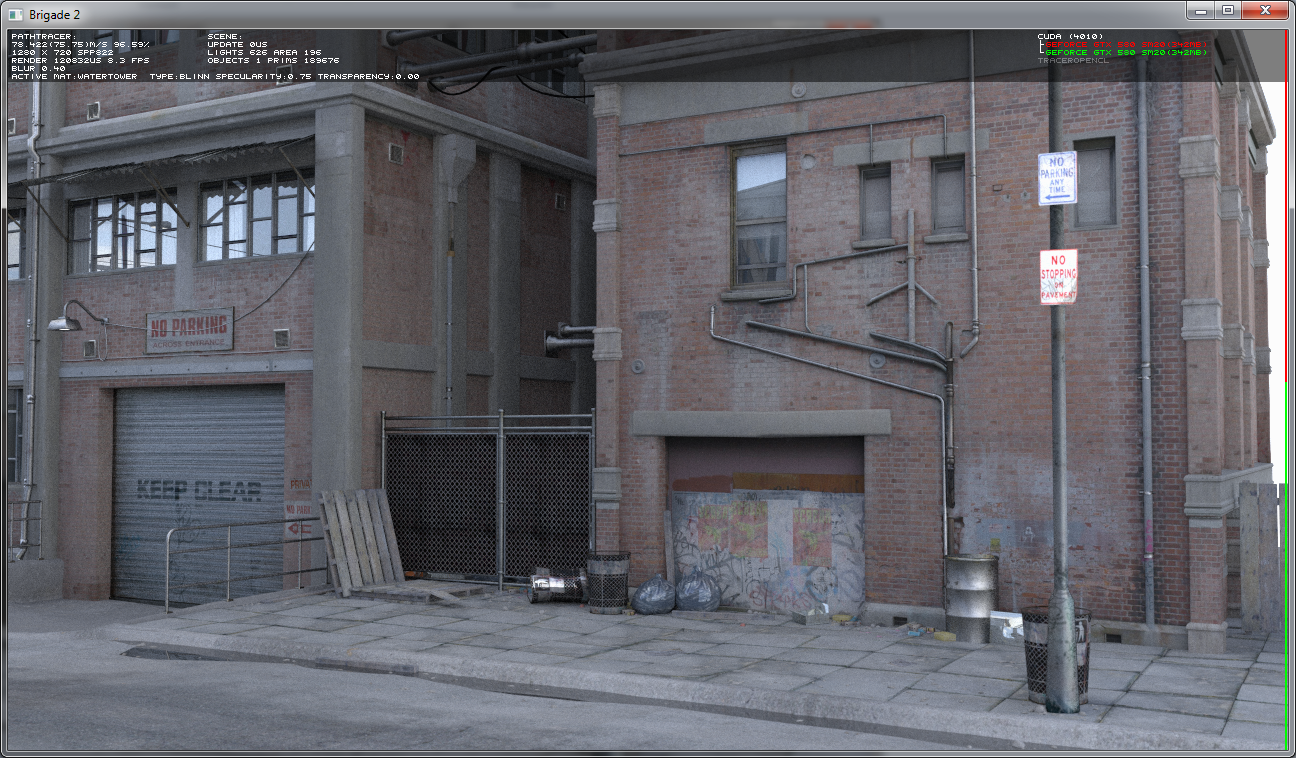
\includegraphics[scale = 0.15]{../figures/hd1.png}
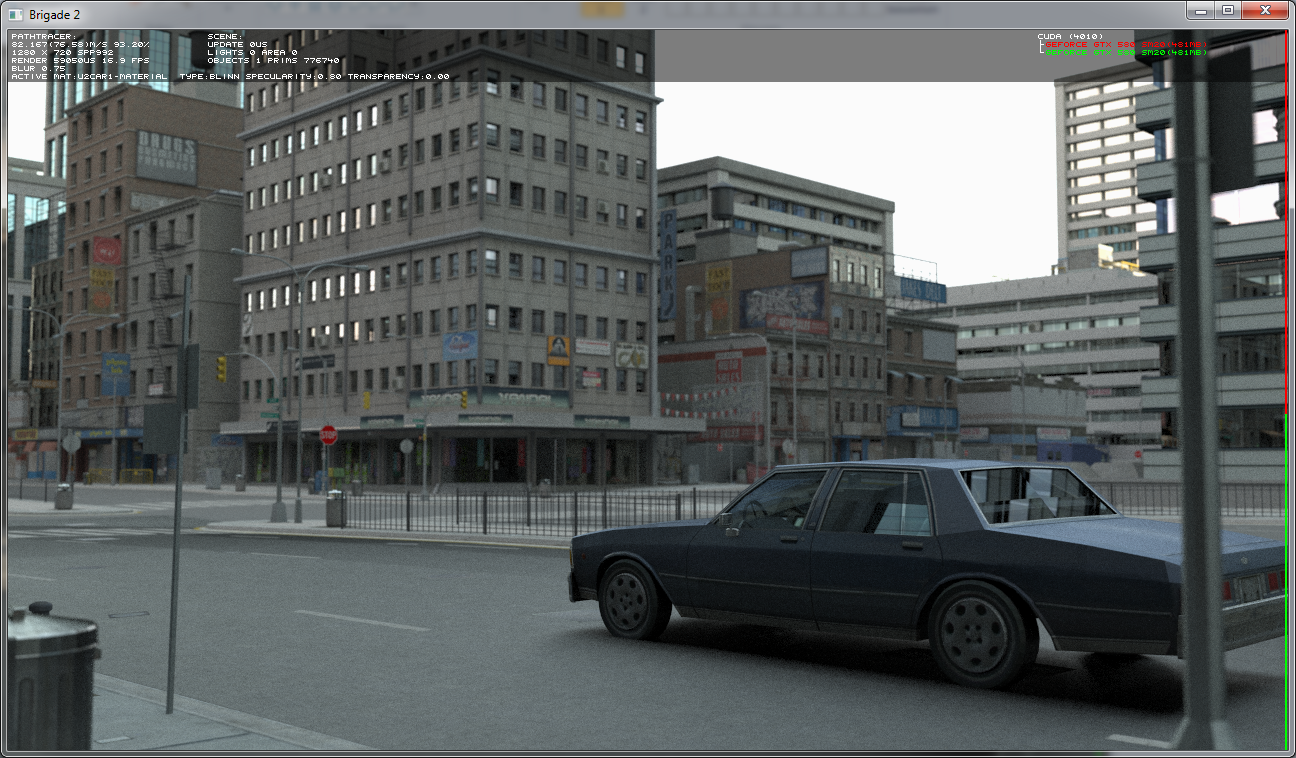
\includegraphics[scale = 0.15]{../figures/blinn5ed.png}

(Imágenes: Brigade 2 Renderer)


\end{frame}




\begin{frame}[Escena]
Cada \textbf{punto} (o píxel) en una imagen de una \textbf{escena} a \textbf{renderizar}, debe computar la \textbf{radiancia} que llega a la \textbf{cámara} desde toda la escena.

Cada objeto de la escena puede emitir radiancia en todo el espectro electromagnético hacia el observador. La radiancia entrante depende de numerosos factores, entre ellos la forma del objeto, el material del objeto, la oclusión existente entre el objeto y la cámara, su temperatura, etc.
\end{frame}



\begin{frame}[Luz]
\begin{block}{Luz}
\begin{itemize}
\item El ser humano evolucionó su comprensión del fenómeno a lo largo del tiempo.
\item Actualmente, se acuña el término ``dualidad onda-partícula'' para describirlo. El mismo es en extremo complejo, por lo tanto debe simplificarse su tratamiento en computación gráfica.
\item La primer simplificación se da teniendo en cuenta que, en la mayoría de los casos sólo la \textbf{luz visible} es la que debe modelarse, ya que la misma define la apariencia del objeto.
\item La distribución de la luz visible en una escena se asume por medio de líneas rectas o \textbf{rayos}, es decir, se opta por la representación óptico geométrica del fenómeno, ya que se representará al mismo a escala macroscópica.
\end{itemize}
\end{block}
\end{frame}

\begin{frame}{}

\centering
%\includegraphics[scale = 0.15]{realidadVirtual.jpg}

\begin{block}{Sin embargo, este es sólo un paso de muchos}
\begin{itemize}
\item Debe modelarse, además, la interacción de la luz con cada objeto en particular.
\item Este problema es aún mayor ya que cada material se comporta de manera diferente.
\item El problema es doble: debe simularse la interacción de la luz con el material \texttt{Y} la geometría del mismo.
\end{itemize}
\end{block}

\end{frame}

\begin{frame}{Materiales}
?`Qué es la apariencia de un material?
\begin{itemize}
\item Definición informal: {\em percepción} del mismo por parte de una persona.
\item Conjunto de estímulos visuales.
%\item Se codifica en datos, estructuras de datos y algoritmos.
\end{itemize}

El \textbf{foto-realismo} busca sintetizar imágenes que produzcan el \textbf{mismo efecto}, en la percepción, que aquél producido por la visualización de una fotografía del material/escena.
\end{frame}
\begin{frame}{Modelado de la Geometría de Materiales}
\begin{itemize}
\item El modelado de cada material depende de la escala buscada.
\item Microscópico: detalles que no son visibles al ojo humano. Se utilizan diversas técnicas estadísticas.
\item Macroscópico: detalles visibles al ojo humano. Se utilizan triángulos, texturas, etc.
\end{itemize}
\end{frame}




\section{Trabajo Previo}

\begin{frame}{Materiales con mayor aparición en escenas}

En computación gráfica, los materiales para los cuales se ha desarrollado mayormente la literatura científica incluye al agua, la piel humana, metales y plásticos, entre otros. Esto se debe a la {\em facilidad del diseño}, a la necesidad de cierto {\em grado de realismo} en el mismo, y a su {\em aparición constante en escenas}.

\end{frame}

\begin{frame}{Materiales con menor aparición en escenas}

Otros materiales, como es el caso de materiales cocidos, materiales porosos y materiales comestibles, poseen un grado de complejidad mayor, debido a varios factores:

\begin{itemize}
\item Geometría compleja y visible, rica interacción con la luz: translucencia, reflexión, absorción, etc.
\item El ser humano puede distinguir con facilidad un modelo si el mismo no es tratado cuidadosamente.
\item El costo computacional de modelar y renderizar estos materiales resultaba excesivo hasta la aparición masiva del hardware paralelo.
\end{itemize}

Alan Fournier: `computer graphics has still not been
able to convincingly render a slice of bread' (2001). 


\end{frame}

\subsection{Técnicas Procedimentales}
\begin{frame}{Técnicas Procedimentales}
Útiles en situaciones donde la supervisión humana repetitiva no es deseable.

Ejemplo, al diseñar un bosque. Diseñar árbol por árbol requeriría un tiempo excesivo.

Debido a esto se desarrollaron técnicas basadas en algoritmos, los cuales permiten diseñar geometrías de manera semiautomática, recibiendo el nombre de \textbf{Procedimentales}.

\end{frame}

\begin{frame}{Sistemas-L}
El botánico Lindenmayer estudió y acuñó estos sistemas para describir la estructura visible de plantas. Fue capaz de representar objetos complejos de manera convincente, utilizando un procedimiento muy sencillo de generación.

La estructura de una planta está representada por medio de una cadena de caracteres.
A través de un procedimiento recursivo de reemplazo de caracteres basados en reglas sencillas, se pueden generar estructuras complejas.

La generación cuenta con un \textbf{axioma}, una o varias reglas \textbf{reglas de producción}, y un \textbf{estado inicial}, indicando posición y orientación.
Además, se especifica un número de iteraciones, donde en cada iteración se aplican reglas de producción a la cadena de caracteres resultante anterior.

Ejemplo:

Axioma: $F$

$P1: F \rightarrow FfF$

Produce las derivaciones:
$F \rightarrow FfF \rightarrow \textbf{FfF}f\textbf{FfF} \ldots$

\end{frame}

\begin{frame}{Sistemas-L: Ejemplo y ``Renderización''}
Dado un estado inicial ($x$,$y$,$90^{\circ}$), el \textbf{axioma} F, y una regla de producción $F \rightarrow FF-FfF-FF$, donde

\begin{itemize}
\item F, moverse hacia adelante un paso $d$, dibujando,
\item f, moverse hacia adelante un paso $d$, sin dibujar,
\item +, rotar un ángulo $\delta$,
\item -, rotar un ángulo $-\delta$.
\end{itemize}

\center
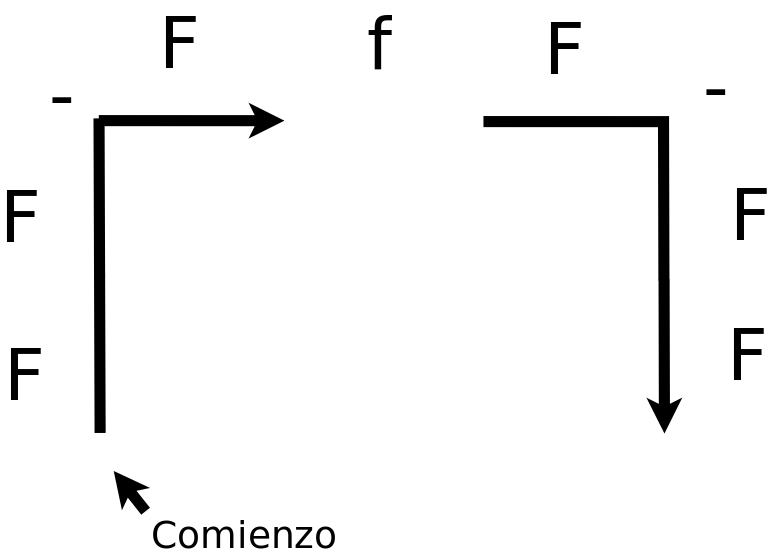
\includegraphics[width=5.8cm]{../figures/tortuga}

\end{frame}

\begin{frame}{Sistemas-L: Arboles}
Por medio de una pila de estados, donde el caracter $[$ se utiliza para copiar el estado actual en la pila (operación {\em push}), y el caracter $]$ implica un reemplazo del estado actual por el de la cabeza de la pila ({\em pop}):


\center
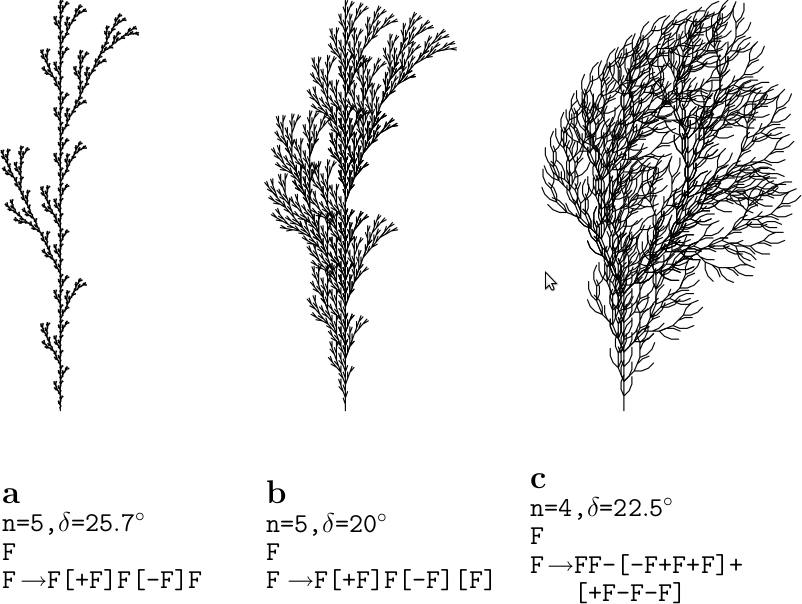
\includegraphics[width=6.3cm]{../figures/sistemalcorchete}

\end{frame}

\begin{frame}{Sistemas-L: Arboles 3D}
\center
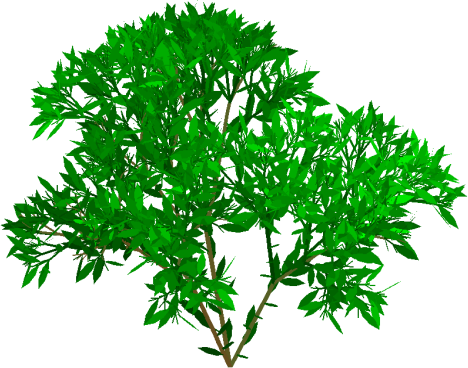
\includegraphics[width=6.3cm]{../figures/3dlsystem}

\end{frame}

\subsection{Modelado Físico de materiales}

\begin{frame}{Modelado Físico de materiales}

Por medio de ecuaciones del comportamiento o crecimiento de los mismos, es posible obtener aproximaciones computacionales más precisas.

Como ejemplo, las ecuaciones de Navier-Stokes se utilizan en la simulación realista de fluídos

Dadas condiciones iniciales para $\bold{u}$ y $p$ cuando $t = 0$, la evolución de las cantidades puede describirse como sigue, independientemente del número de dimensiones,

\begin{align*}
\nabla \cdot \bold{u} &= 0\\
\frac{\partial \bold{u} }{\partial t} &= - (\bold{u} \cdot \nabla) \bold{u} - \frac{1}{\rho} \nabla p + \nu \nabla^{2} \bold{u} + \bold{f},
\end{align*}

\noindent donde $\nu$ representa la viscosidad cinemática del fluido, $\rho$ la densidad y $\bold{f}$ una fuerza externa.

\end{frame}

\begin{frame}{Ecuaciones de Navier-Stokes, humo}
\center
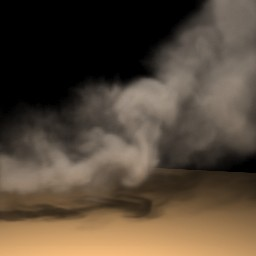
\includegraphics[width=6.3cm]{../figures/smoke}

\end{frame}

\subsection{Renderizado}


\begin{frame}{Ecuación del Renderizado}
La misma modela la radiancia entrante en un punto $x$ por medio de todas las superficies $s_{i}$ de la escena, pasando por todos los puntos $x'$ de todas las superficies.
\begin{equation*}
L(\bold{x'} \rightarrow \bold{x}) =  g(\bold{x'}  \rightarrow \bold{x})  \left[ \epsilon(\bold{x'}  \rightarrow \bold{x}) + \int_{s}{\rho(\bold{x''}  \rightarrow \bold{x'}  \rightarrow \bold{x})L(\bold{x''}  \rightarrow \bold{x}) d\bold{x''}} \right]
\end{equation*}
donde $L(\bold{x'} \rightarrow \bold{x})$ representa la intensidad de la luz que viaja del punto tridimensional $\bold{x'}$ al punto $\bold{x}$ (sin oclusiones), $g(\bold{x'} \rightarrow \bold{x})$ un termino geométrico que modela la oclusión que podría existir entre $\bold{x}$ y $\bold{x'}$, $\epsilon(\bold{x'} \rightarrow \bold{x})$ la intensidad de la luz emitida desde $\bold{x'}$ a $\bold{x}$, $\rho(\bold{x''}  \rightarrow \bold{x'}  \rightarrow \bold{x})$ la intensidad de la luz emitida de $\bold{x''}$ a $\bold{x}$ por medio de una superficie en $\bold{x'}$ (esta cantidad será llamada función bidireccional de distribución de reflectancia, BRDF), y $S=\bigcup{s_{i}}$ la unión de todas las superficies $s_{i}$ de la escena
\end{frame}

\begin{frame}{Ecuación del Renderizado}
\begin{wrapfigure}{l}{6cm}
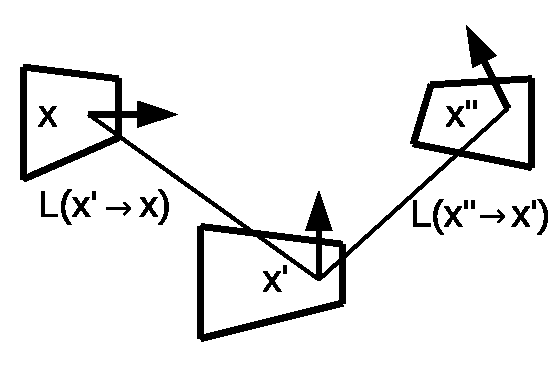
\includegraphics[scale = 0.6]{../figures/rendequation}
\end{wrapfigure}

Puede observarse que la ecuación presenta una definición recursiva, ya que la energía radiante saliente de un punto $x'$ depende de la energía radiante que llega desde todos los puntos de todas las superficies a ese punto.
De esta forma, $\bold{x}$,$\bold{x'}$ y $\bold{x''}$ varían sobre todas las superficies de la escena.
Además se asume una superficie $S_{0}$, la cual se modela como una semi-esfera que engloba a toda la escena.

La ecuación aproxima las propiedades óptico-geométricas de las ecuaciones del electromagnetismo de Maxwell.
\end{frame}


\begin{frame}{Ecuación del Renderizado de Volúmenes}
\begin{equation*}
\begin{aligned}
(\vec{\omega} \cdot \nabla) L(\bold{x} \rightarrow \vec{\omega}) = - \sigma_{a}(\bold{x}) L(\bold{x} \rightarrow \vec{\omega}) - \sigma_{s}(\bold{x}) L(\bold{x} \rightarrow \vec{\omega}) + \\
\sigma_{a}(\bold{x}) L_{e}(\bold{x} \rightarrow \vec{\omega}) + \sigma_{s}(\bold{x}) L_{i}(\bold{x} \rightarrow \vec{\omega}).
\end{aligned}
\end{equation*}
donde $\sigma_{a}$: coeficiente de absorción del medio, $\sigma_{s}$: coeficiente de dispersión del medio.
La misma expresa que el cambio ($\nabla$) de radiancia $L$ de un rayo de luz en un medio, en una dirección dada ($\vec{\omega}$) está dado por cuatro fenómenos: absorción, dispersión saliente, emisión (del medio) y dispersión entrante.
\end{frame}

\begin{frame}{Ecuación del Renderizado de Volúmenes}
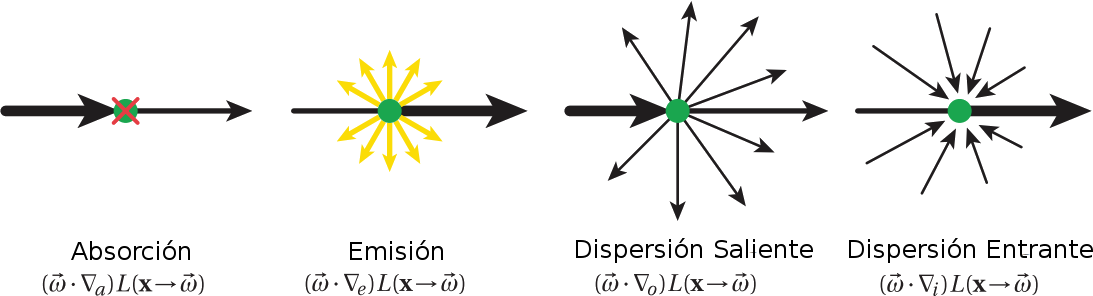
\includegraphics[scale = 0.6]{../figures/fenomenosrte}
\end{frame}



\subsection{Materiales porosos}
\begin{frame}{Materiales porosos - Trabajo Previo}
Los modelos actuales de generación de geometría de materiales porosos en el área resultan de procesos artísticos.
Se utilizan diversos ruidos, como los ruidos de Voronoi, Perlin y Worley. Sin embargo, los métodos deben combinarse con otras consideraciones ad-hoc.

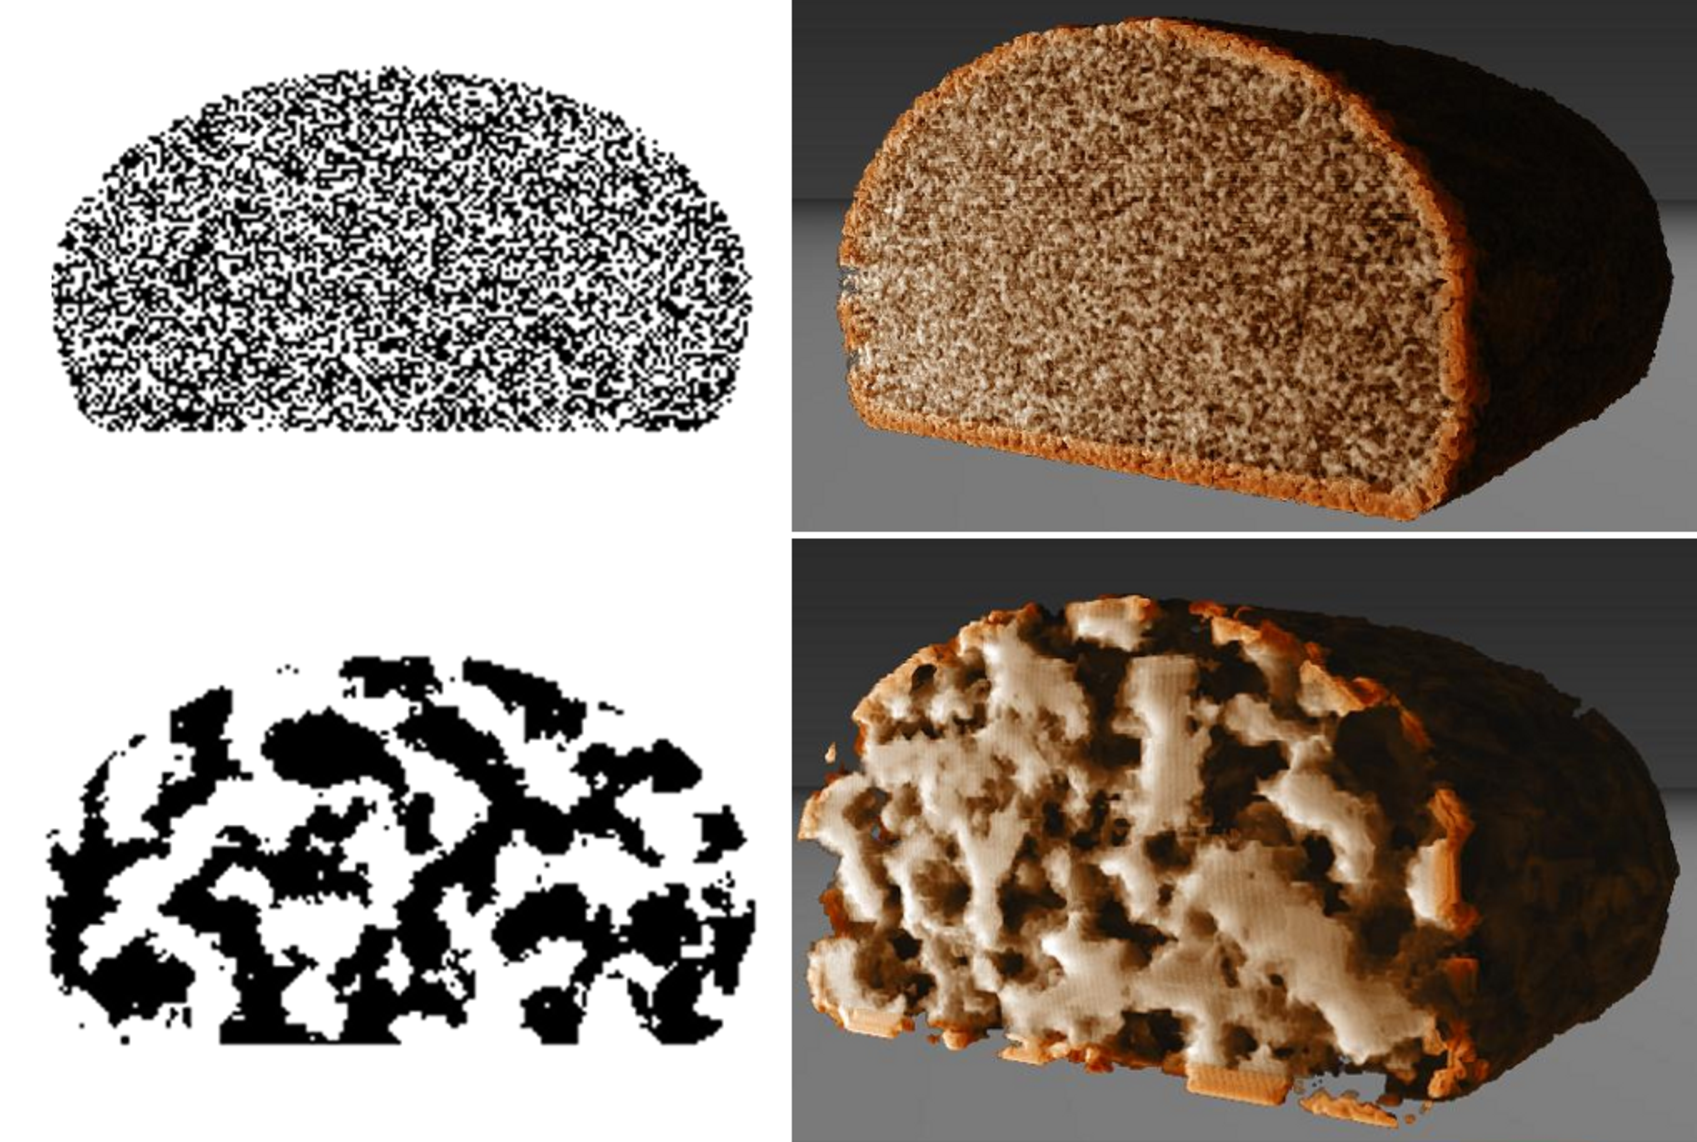
\includegraphics[scale = 0.2]{../figures/Fig8}
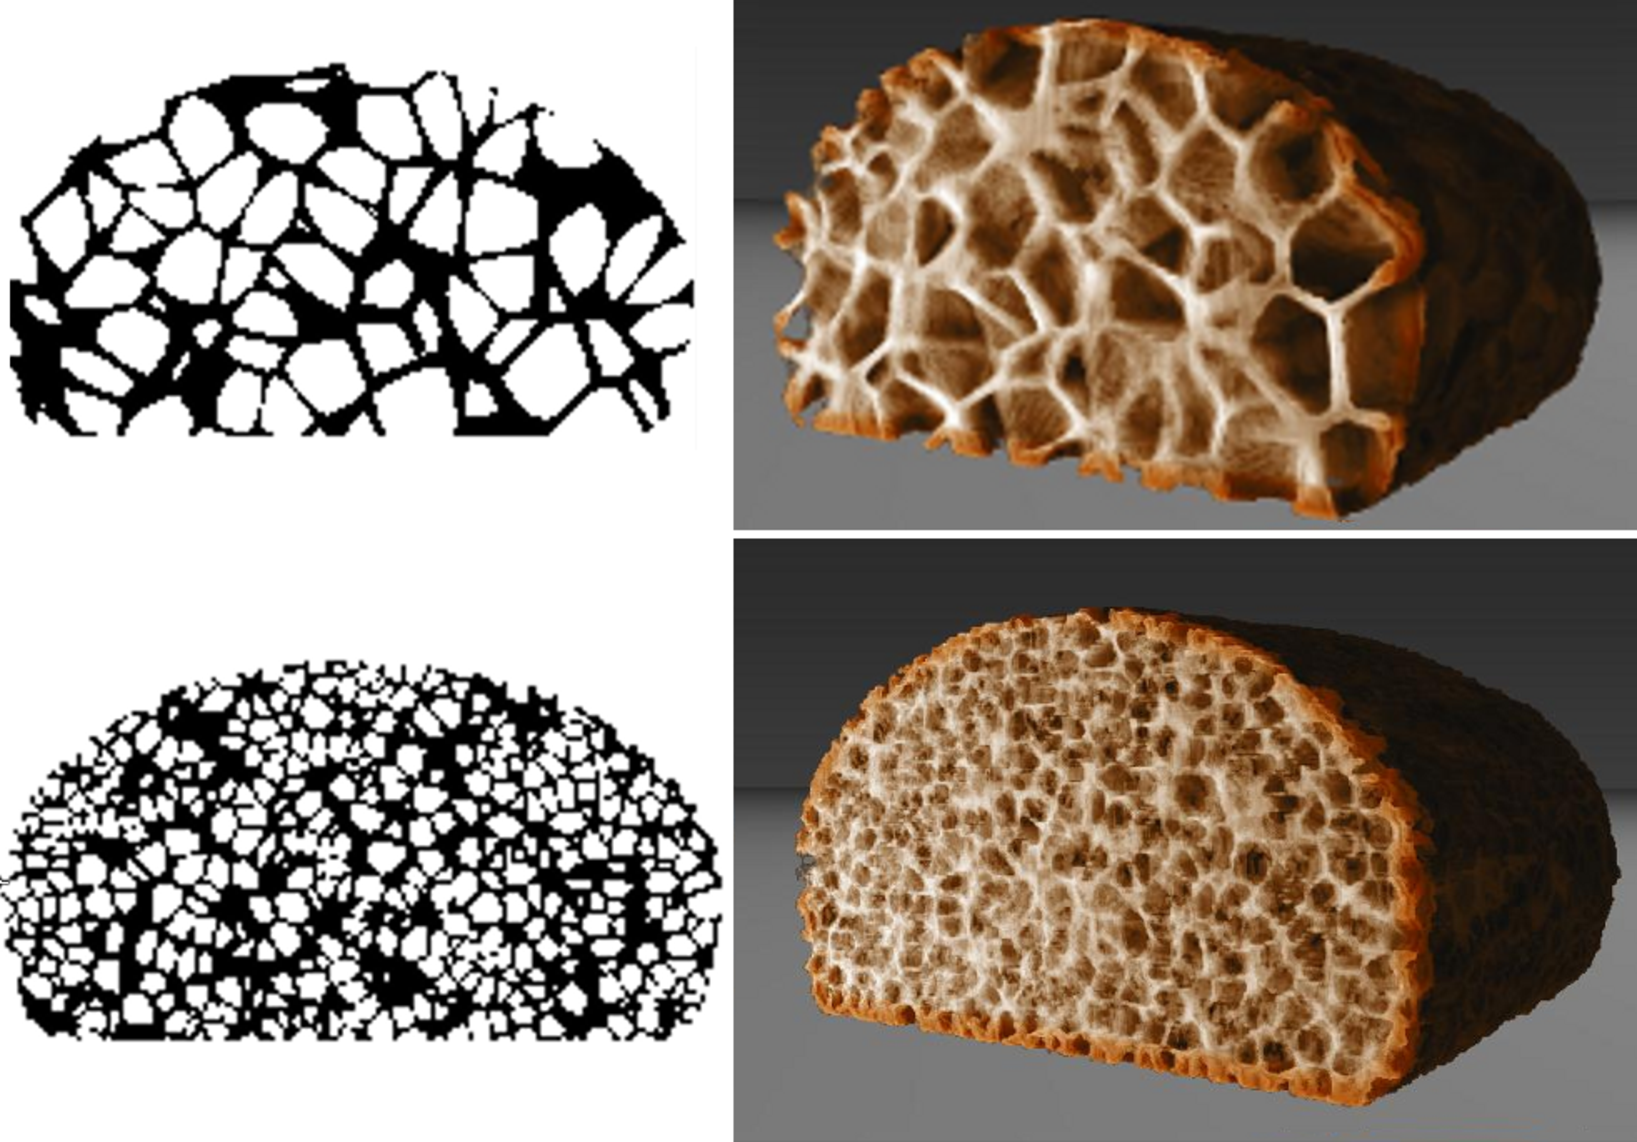
\includegraphics[scale = 0.2]{../figures/Fig9CAVW}

Ratatouille (Película): modelo de pan basado en ruido de Voronoi + un mapa indicando deformación de burbujas.
\end{frame}

\begin{frame}{Materiales porosos - Trabajo Previo}
Desventajas: 
\begin{itemize}
\item control sobre cantidad y tamaño de las burbujas
\item deformación de burbujas
\item el usuario debe ser experto
\end{itemize}

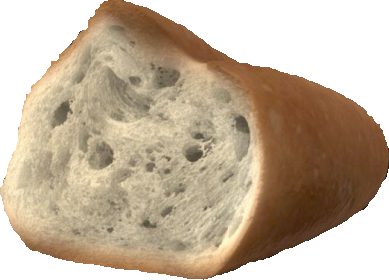
\includegraphics[scale = 0.3]{../figures/ratatouille}

\end{frame}

\begin{frame}

Modelo fenomenológico: Tong et al (2005), "Modeling and Rendering of quasi-homogeneous Materials"

Capturas sobre materiales reales utilizando cámaras y lásers $\rightarrow$ se obtienen distribuciones precisas de radiancia en el material.

\begin{itemize}
\item Proceso de captura muy complejo
\item Limitado a una geometría
\item Tiempos de cómputo no claramente establecidos
\item Imposibilidad de realizar cortes
\end{itemize}

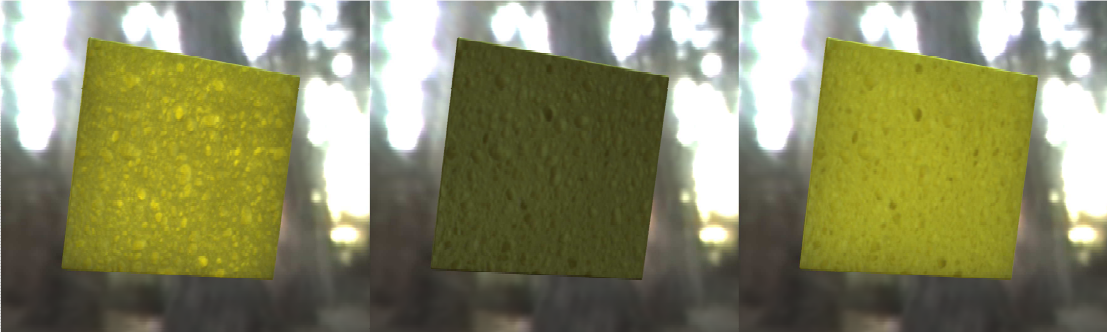
\includegraphics[scale = 0.3]{../figures/esponja}

\end{frame}


\section{Modelado de Geometrías Porosas}
\subsection{Modelado de Geometrías Porosas}
\begin{frame}{Propuesta}
Presentamos un modelo de generación de geometrías porosas basados en:
\begin{itemize}
\item Sistemas de Partículas que crecen, evitándose
\item Sistemas dinámicos como medio de crecimiento
\end{itemize}
\end{frame}

\begin{frame}{Sistemas de partículas}
Características
\begin{itemize}
\item Conjunto de \textbf{partículas}: una partícula posee posición, dirección, color, tiempo de vida, etc.
\item Utilizado para representar fluídos, y objetos con interfaces sin definición precisa

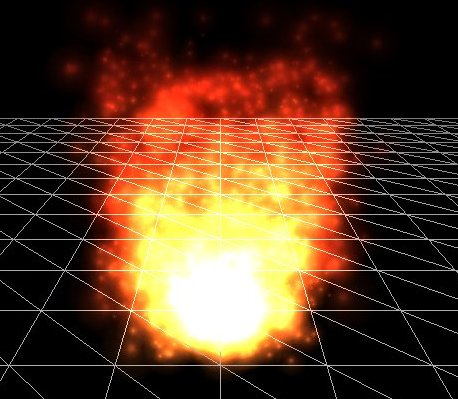
\includegraphics[scale = 0.3]{../figures/fire}
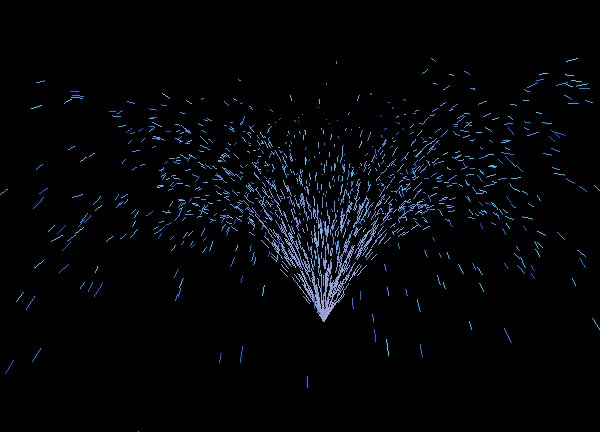
\includegraphics[scale = 0.277]{../figures/fireworks}
\end{itemize}
\end{frame}

\begin{frame}
El sistema consta de un conjunto de partículas $P$, y dos grillas, $L$, y $L^{2}$:
\begin{align*}
  P = \{p_{1}, ... , p_{n}\}, n  \in \mathbb{N}, \\
  L_{N\times N \times N},\\
  L^{2}_{N\times N \times N},\\ N \in \mathbb{N}.
\end{align*}

inicialmente $L_{xyz}=1$: masa

inicialmente $L^{2}_{xyz}=-1$: celda libre,

Cada partícula posee:
\begin{equation*}
  p_{i} = \{O_{i}, C_{i}\}, 1 \le i \le n,
\end{equation*}

\begin{itemize}
\item $O_{i} = \{o_{1}, ... , o_{n_{i}}\}$:posiciones ocupadas por la part\'icula en $L$.

\item $C_{i} = \{c_{1}, ... , c_{m_{i}}\}$:posiciones en el {\em contorno} de la part\'icula en $L$.
\end{itemize}

\end{frame}

\begin{frame}{Ejemplo: crecimiento}
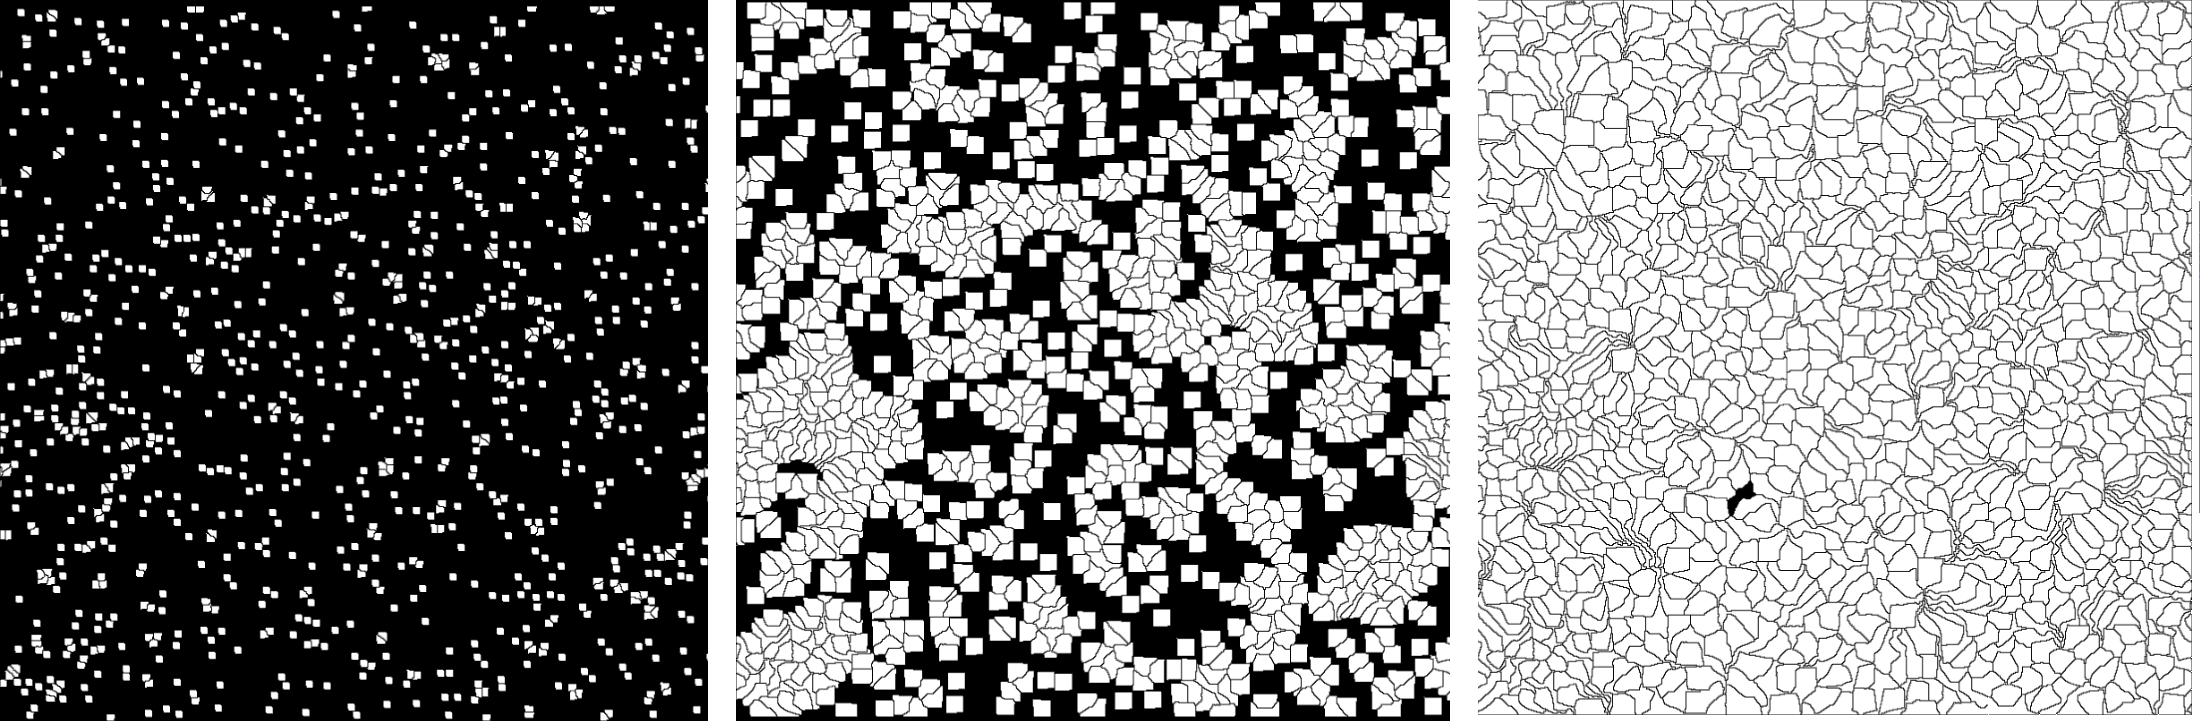
\includegraphics[scale = 0.15]{../figures/modeladocrec}
\end{frame}


\begin{frame}{Sistemas dinámicos}

De manera general, las ODEs se representan utilizando el siguiente sistema de ecuaciones:
\begin{equation*}
  \begin{aligned}
    \dot{x_{1}} = f_{1}(x_{1},\ldots,x_{n}),\\
    \ldots\\
    \dot{x_{n}} = f_{n}(x_{1},\ldots,x_{n}),
  \end{aligned}
\end{equation*}

Ejemplo en dos dimensiones (imagen de la izquierda),
\begin{equation*} \label{eq:simple}  
  \begin{aligned}
    \dot{x} &= x^{2}-y^{2}+1,\\
    \dot{y} &= 2xy+1.
  \end{aligned}
\end{equation*}

\end{frame}

\begin{frame}{Sistemas Dinámicos}
  \centerline{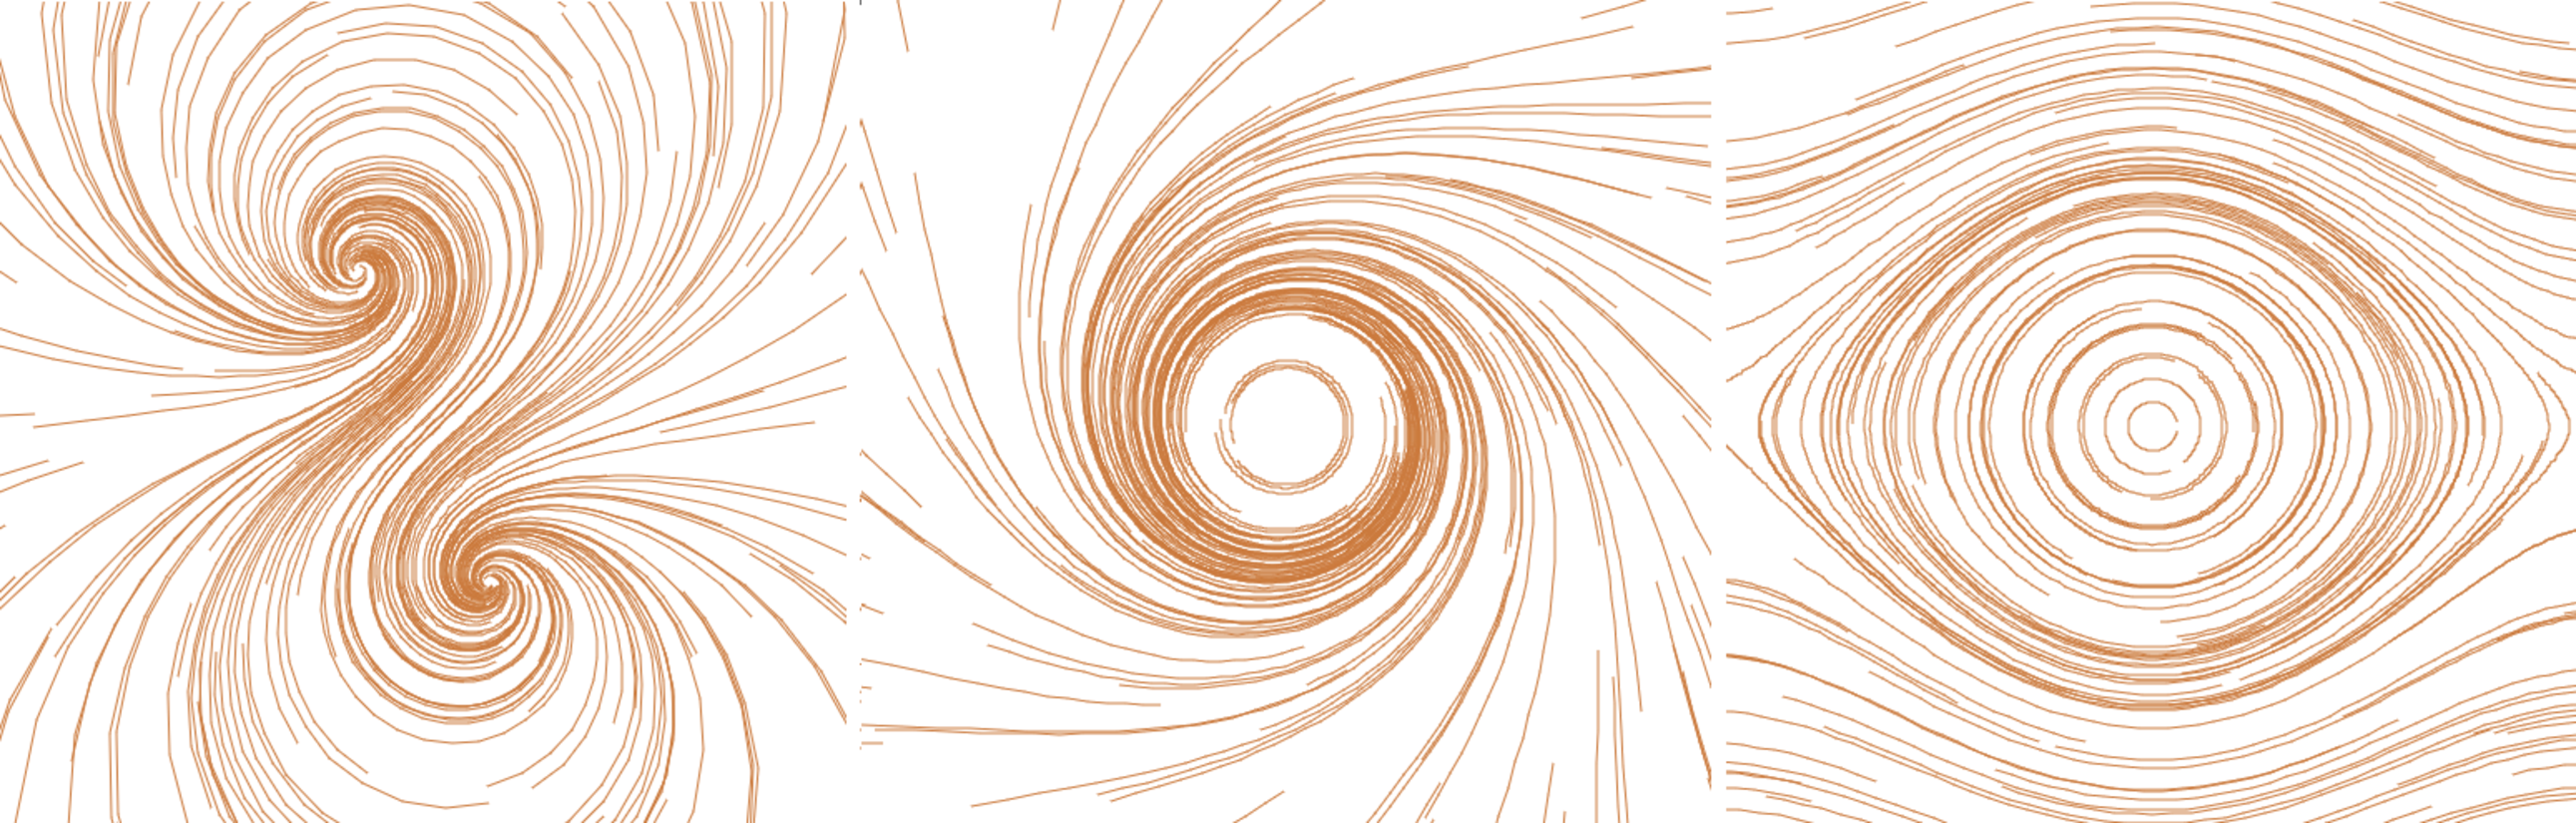
\includegraphics[width=12cm]{../figures/Fig2}}
\end{frame}

\begin{frame}{Sistemas de partículas + Sistemas Dinámicos}
Utilizando distintos parámetros de aleatoriedad en el crecimiento, se obtienen distintas apariencias
  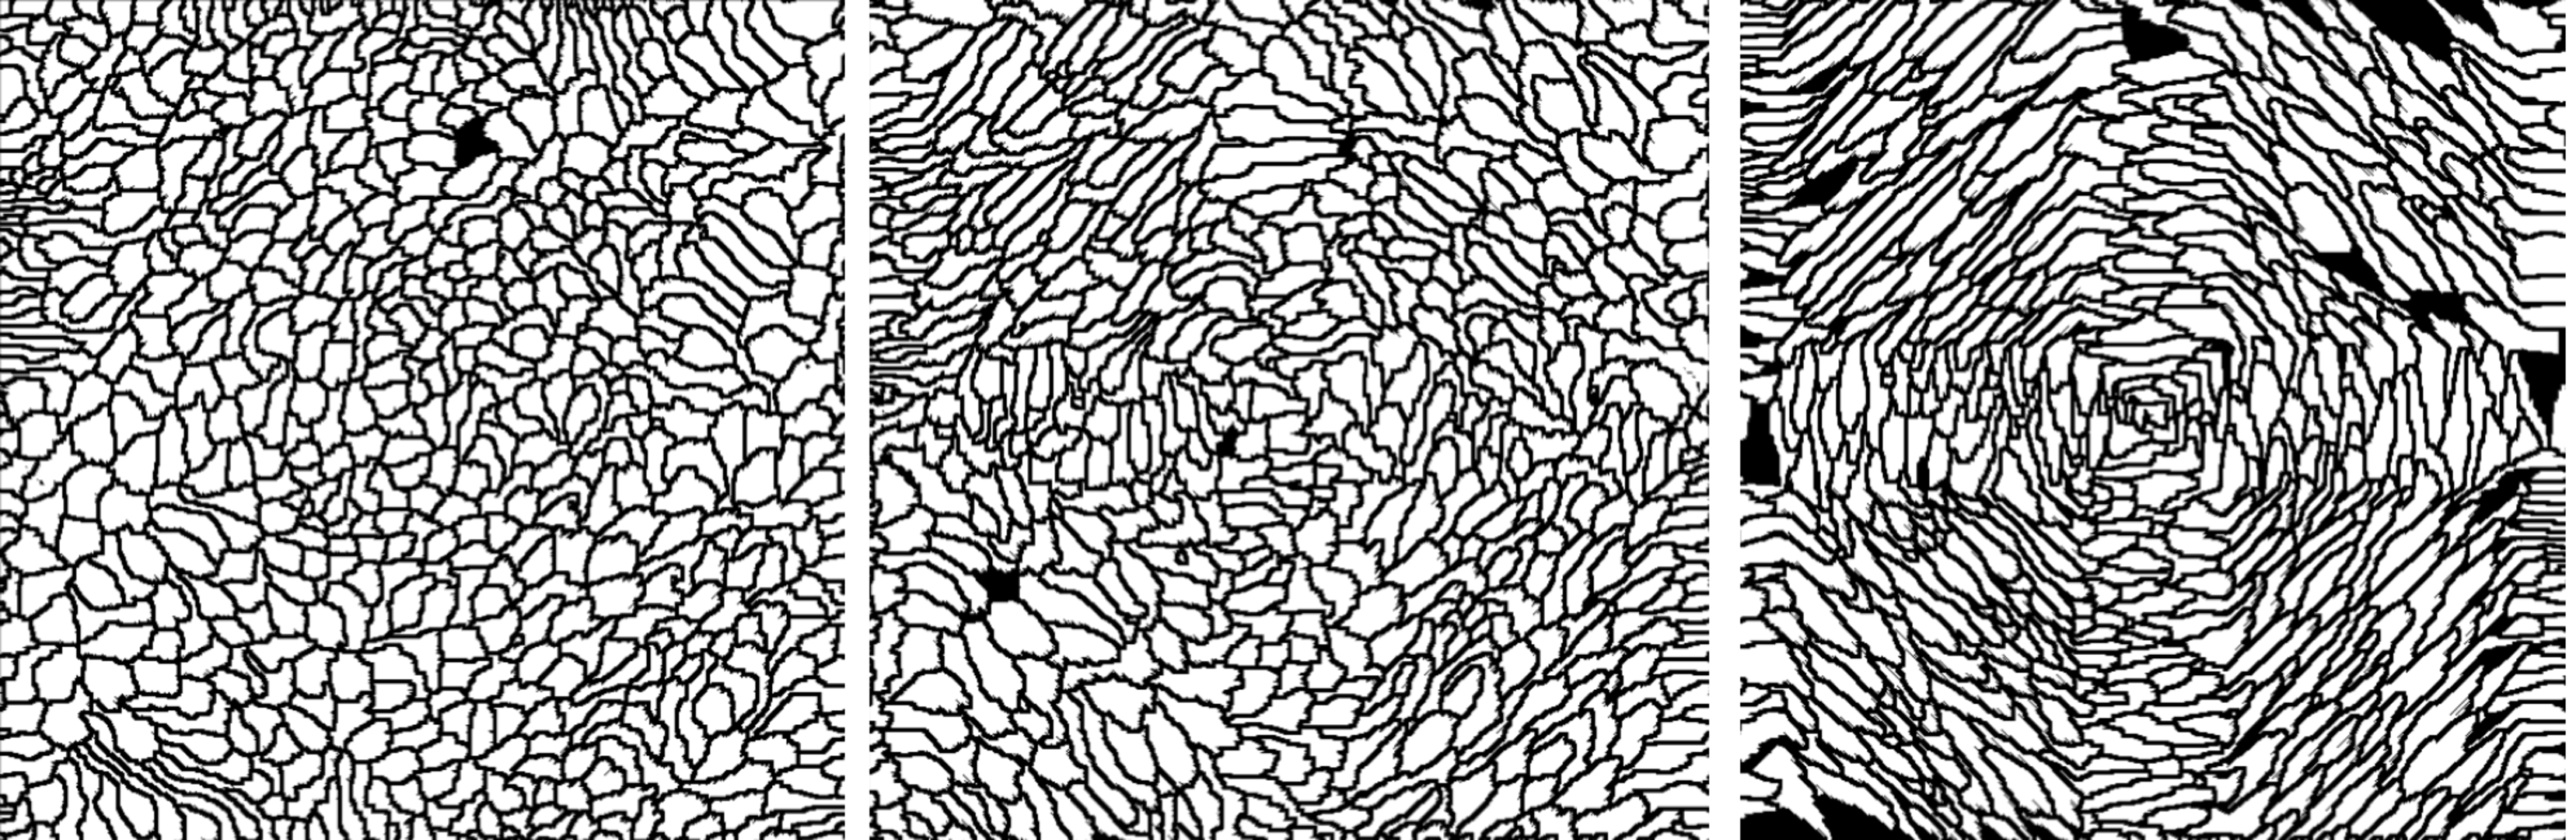
\includegraphics[width=12cm]{../figures/Fig3}
\end{frame}

\begin{frame}{Condiciones de contorno}
Dada una geometría tridimensional arbitraria, se elige un eje Cartesiano ($x$, $y$ o $z$) y se computan cortes bidimensionales sobre ese eje.

Para cada corte se establecen condiciones de contorno, estableciendo un campo vectorial discreto que ``sigue'' al contorno: ortogonal al gradiente del corte.

  \centerline{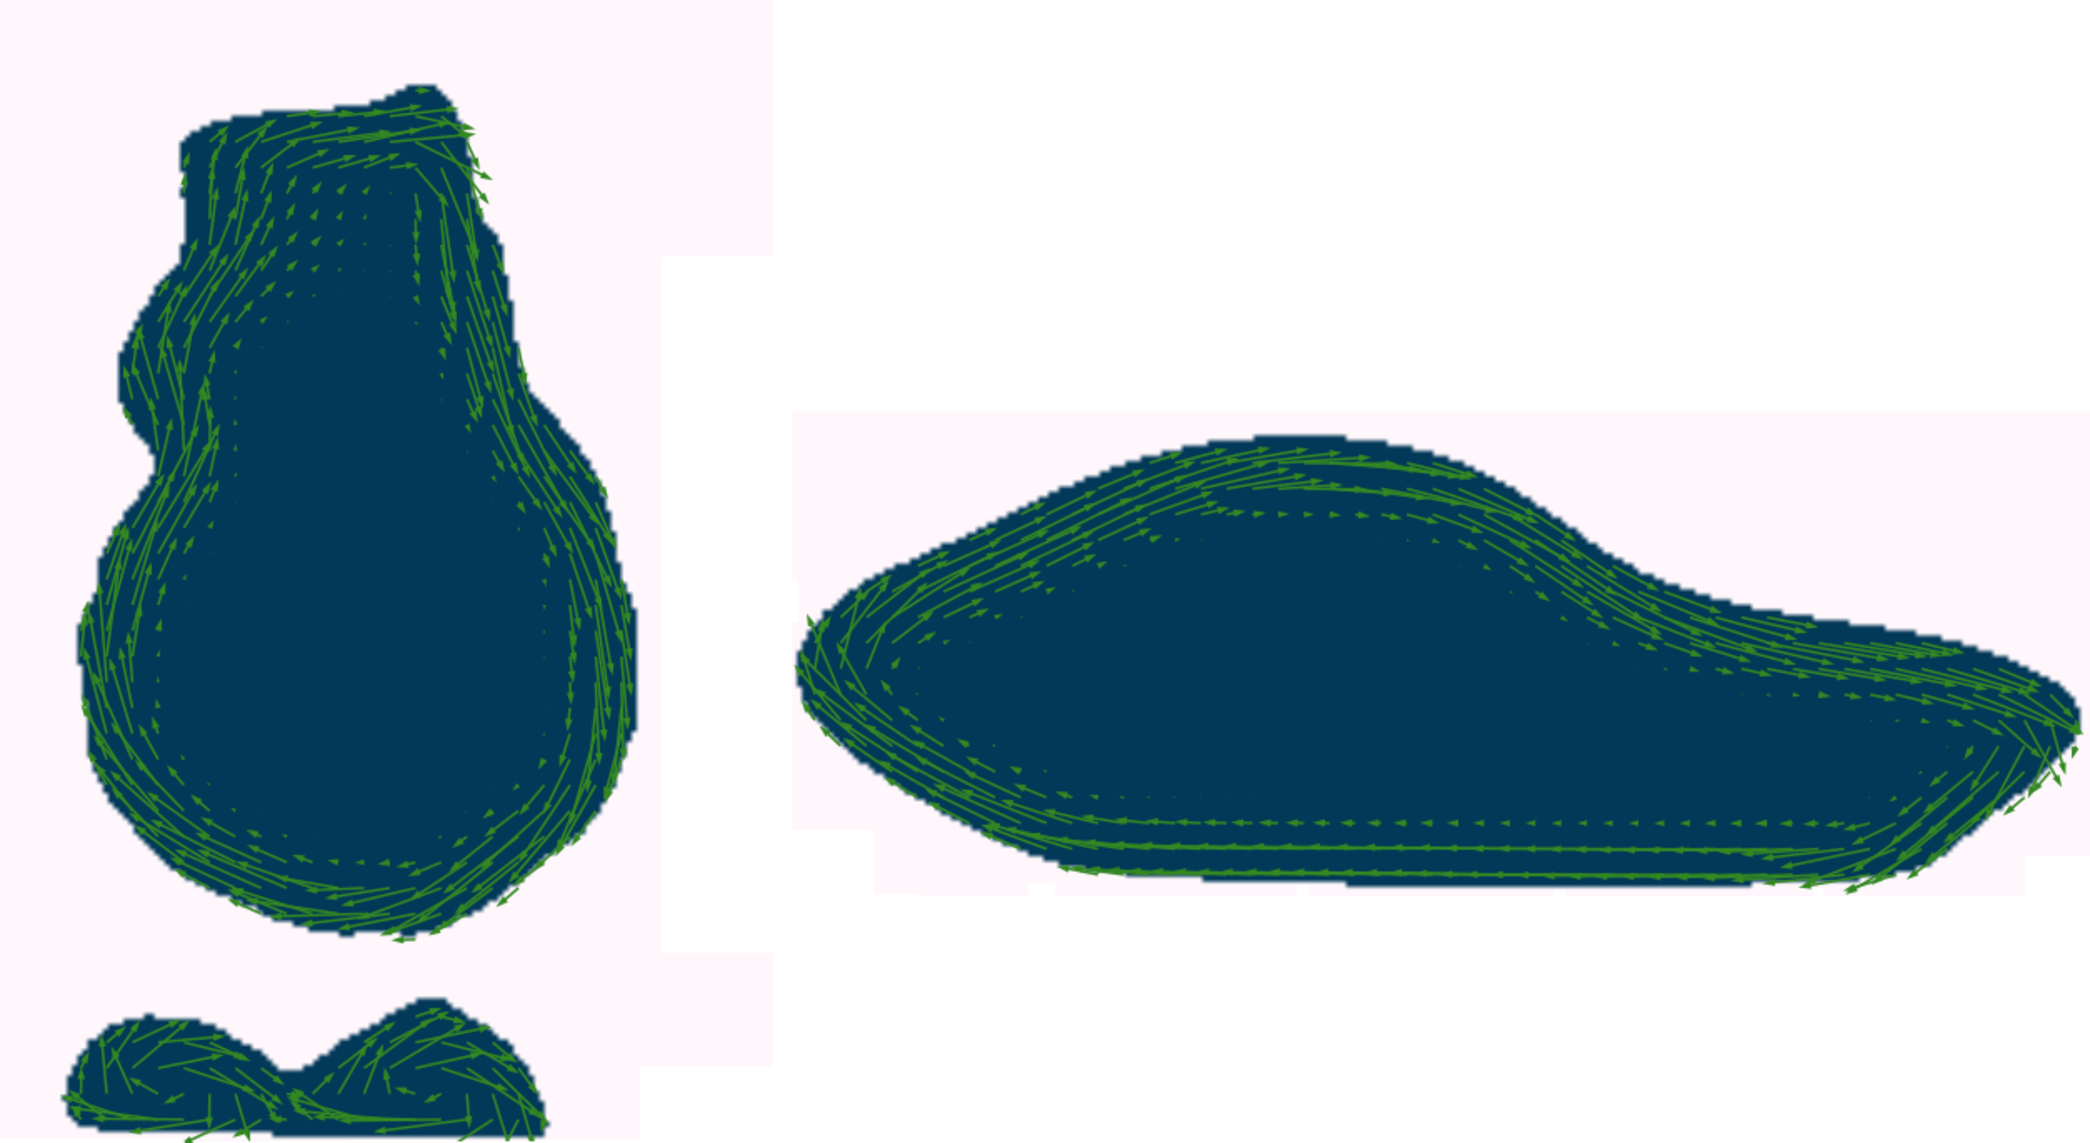
\includegraphics[width=8cm]{../figures/Fig4}}
\end{frame}

\begin{frame}{Resultados}
Finalmente se centra el sistema dinámico en el {\em centro de masa} de cada corte, y junto a las condiciones de contorno, definen un patrón natural para el corte.

Si bien esta elección no representa una parametrización completamente tridimensional, resulta más intuitivo definir un sistema dinámico en dos dimensiones.

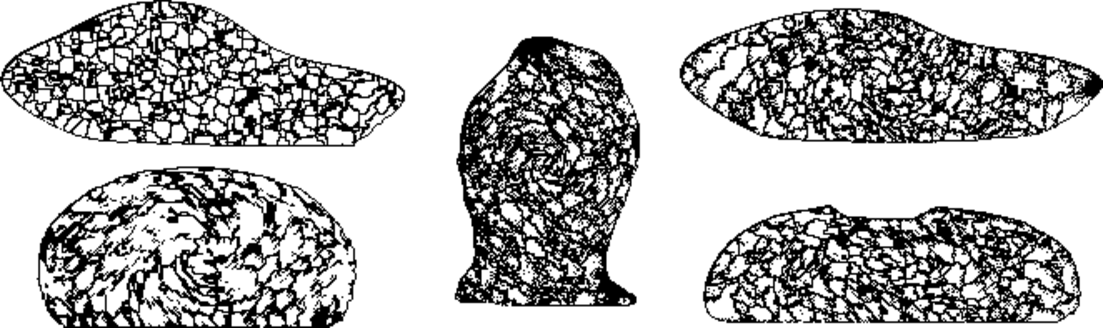
\includegraphics[width=12cm]{../figures/Fig5}
\end{frame}

\begin{frame}{Resultados}
\centerline{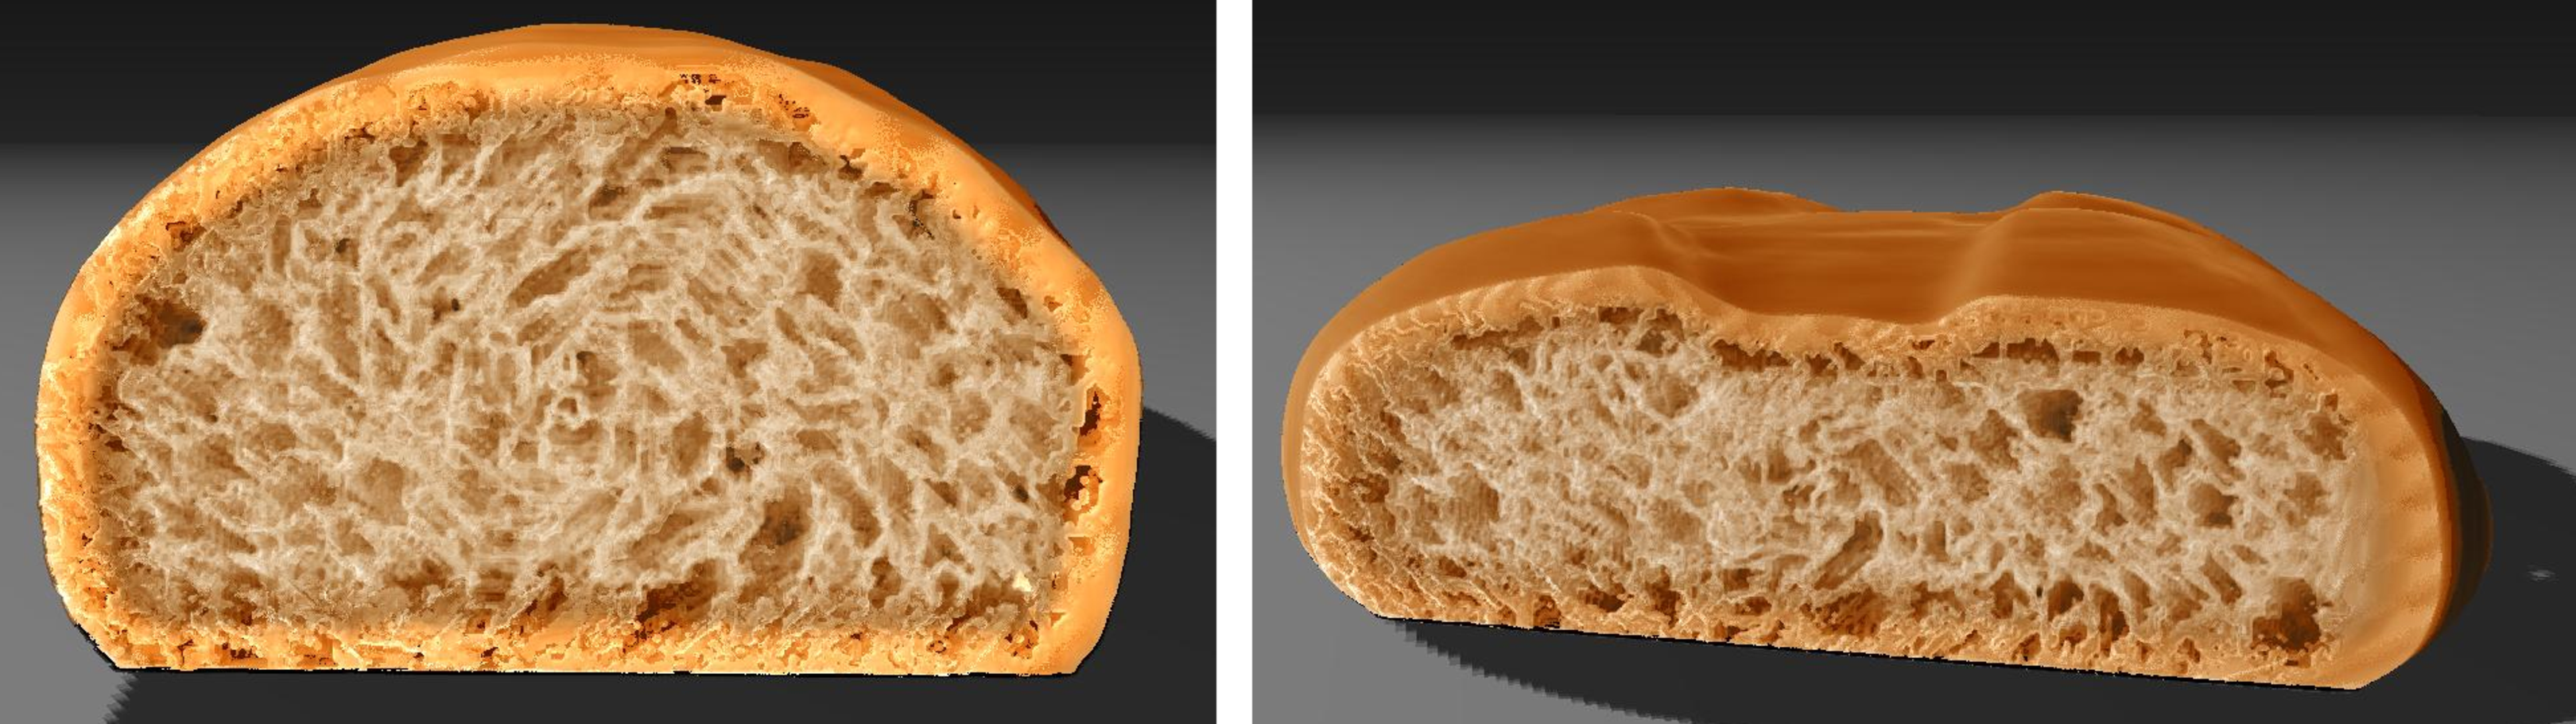
\includegraphics[width=10cm]{../figures/Fig11CAVW}}


Sistemas dinámicos adaptativos (dependiendo del ancho y alto del corte).

\centerline{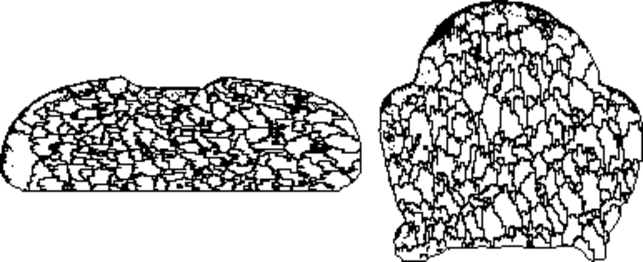
\includegraphics[width=7cm]{../figures/Fig6}}

\end{frame}

\begin{frame}{Resultados}
Parámetro {\em separación} = 2 entre partículas

\centerline{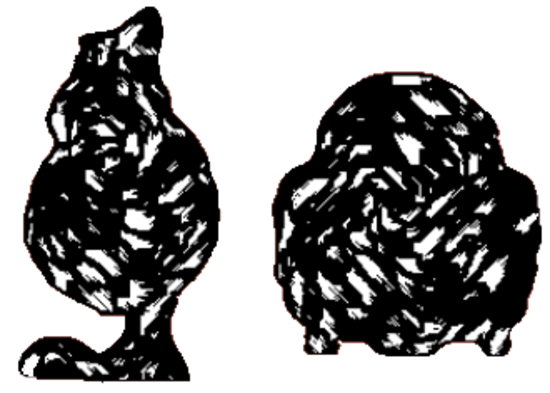
\includegraphics[width=8cm]{../figures/Fig7}}
\end{frame}

\begin{frame}{Renderizados}

\centerline{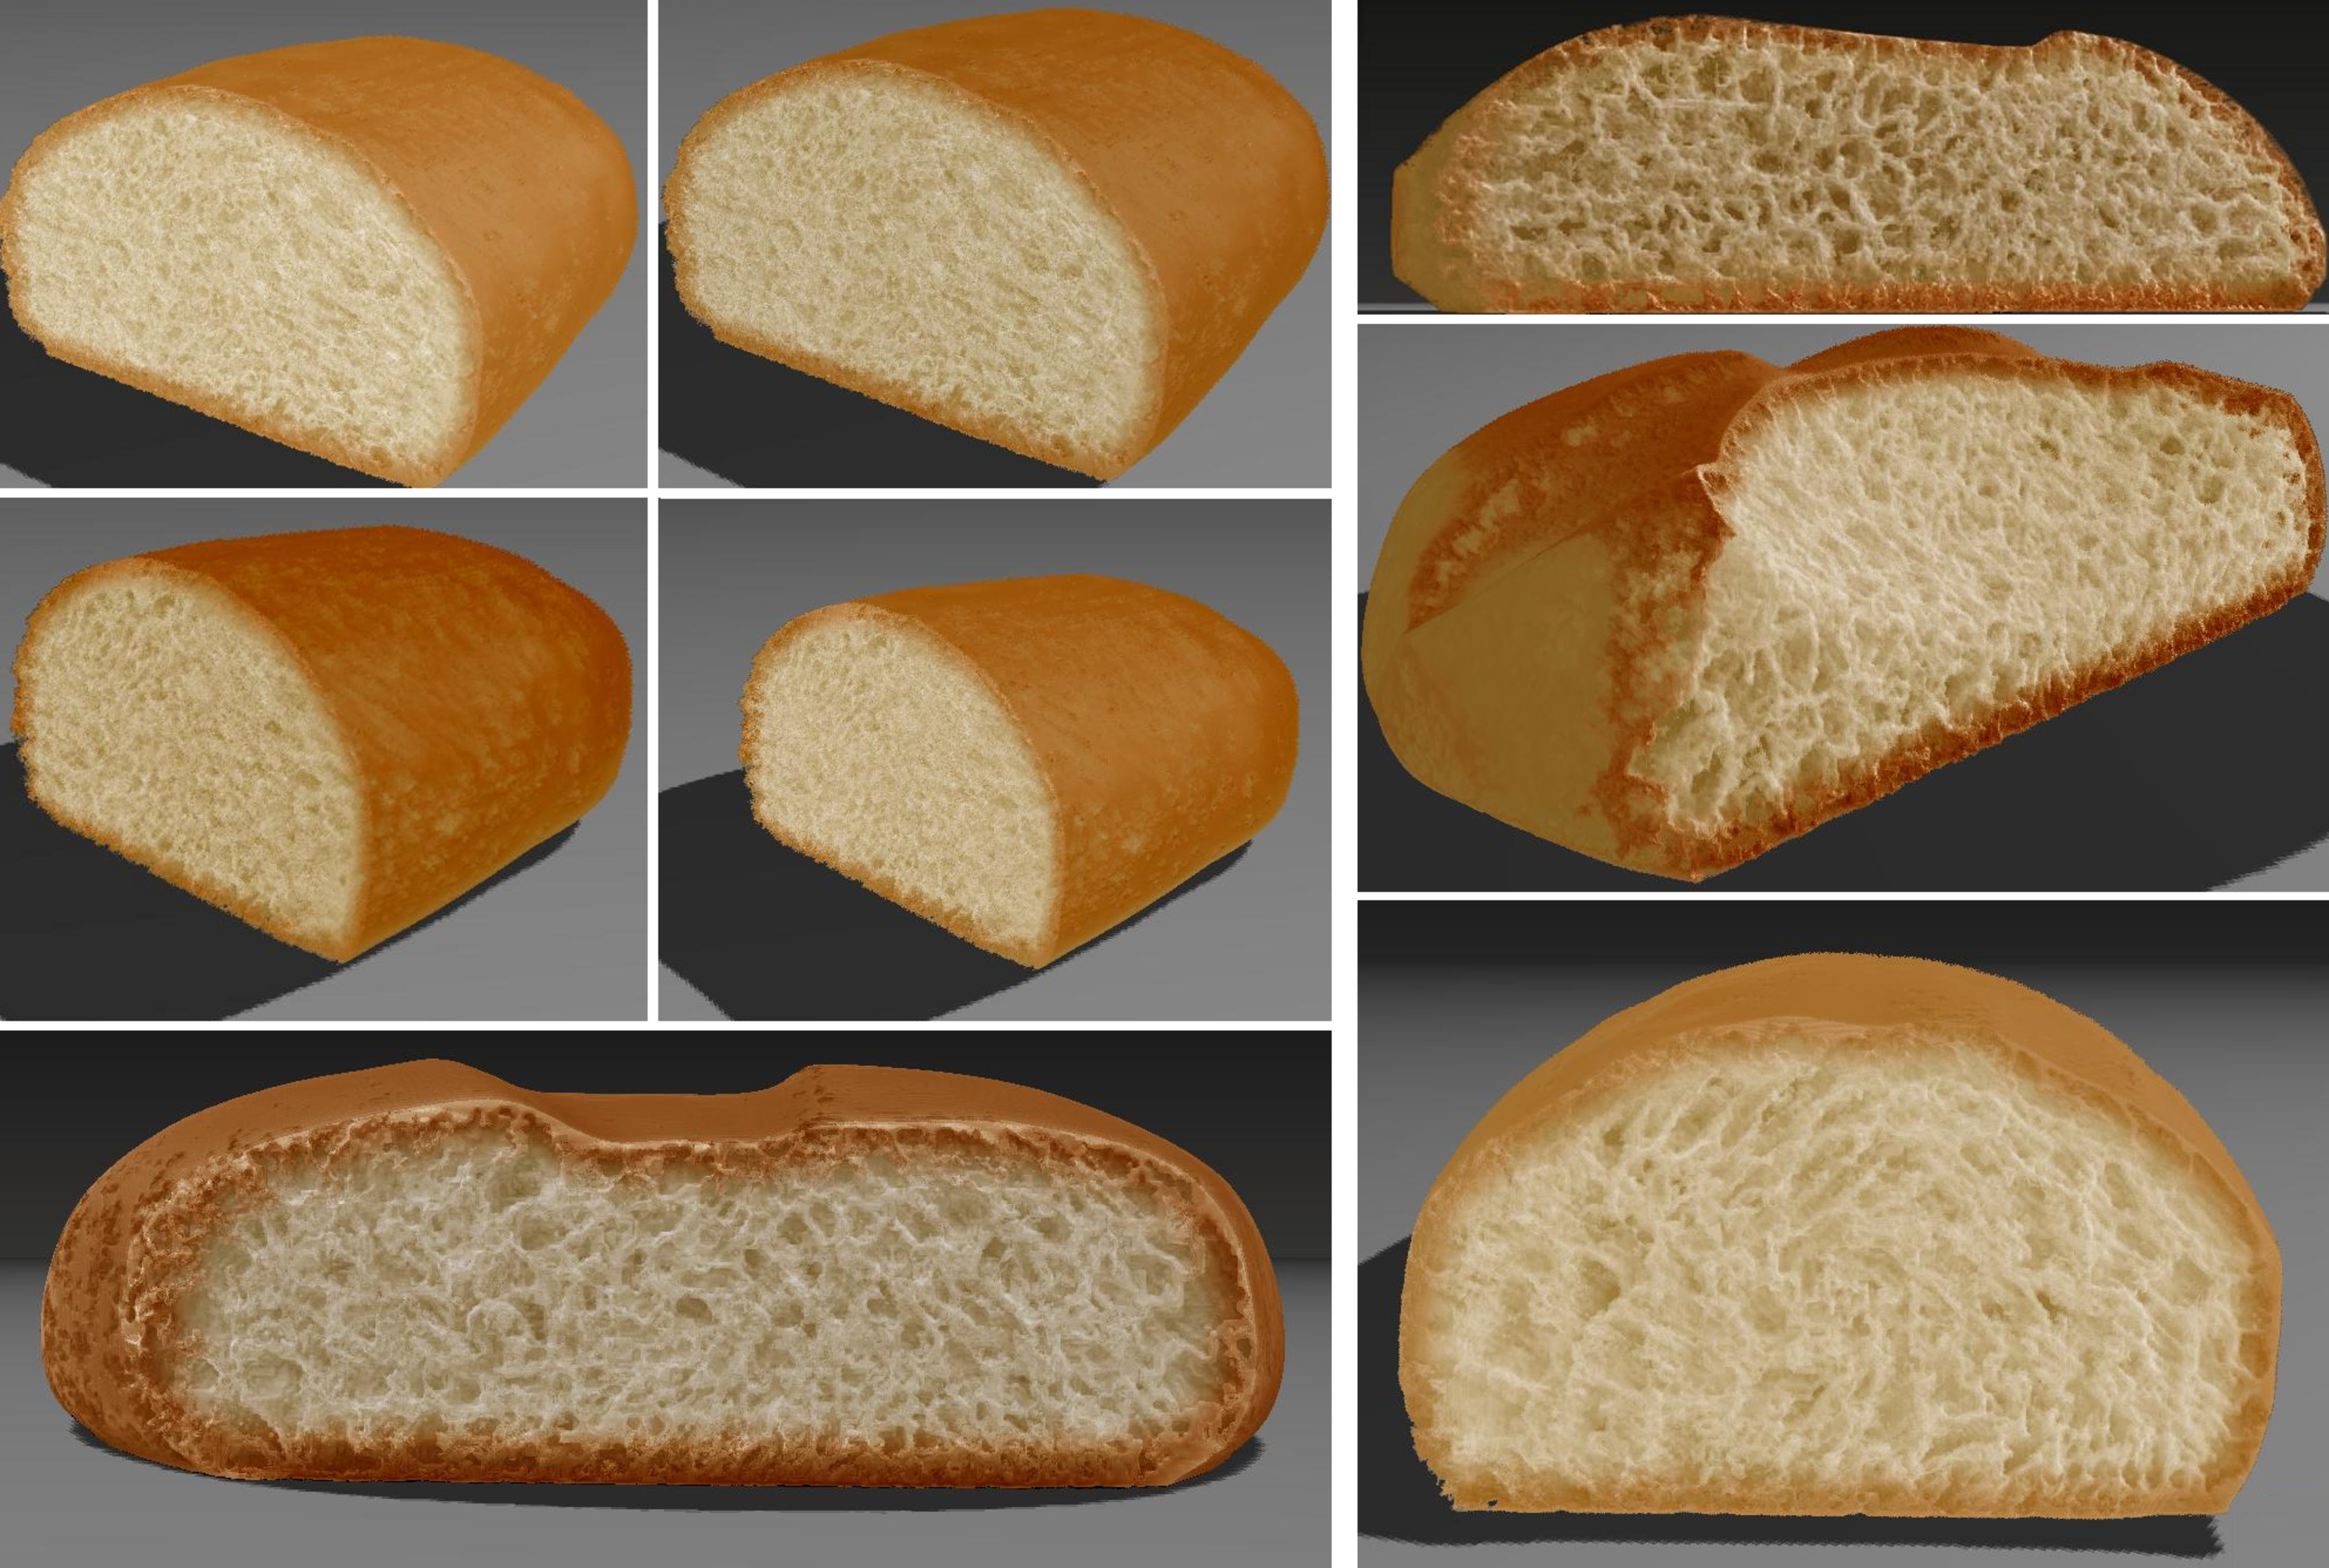
\includegraphics[width=10cm]{../figures/Fig12CAVW}}
\end{frame}

\begin{frame}{Esponjas}

\centerline{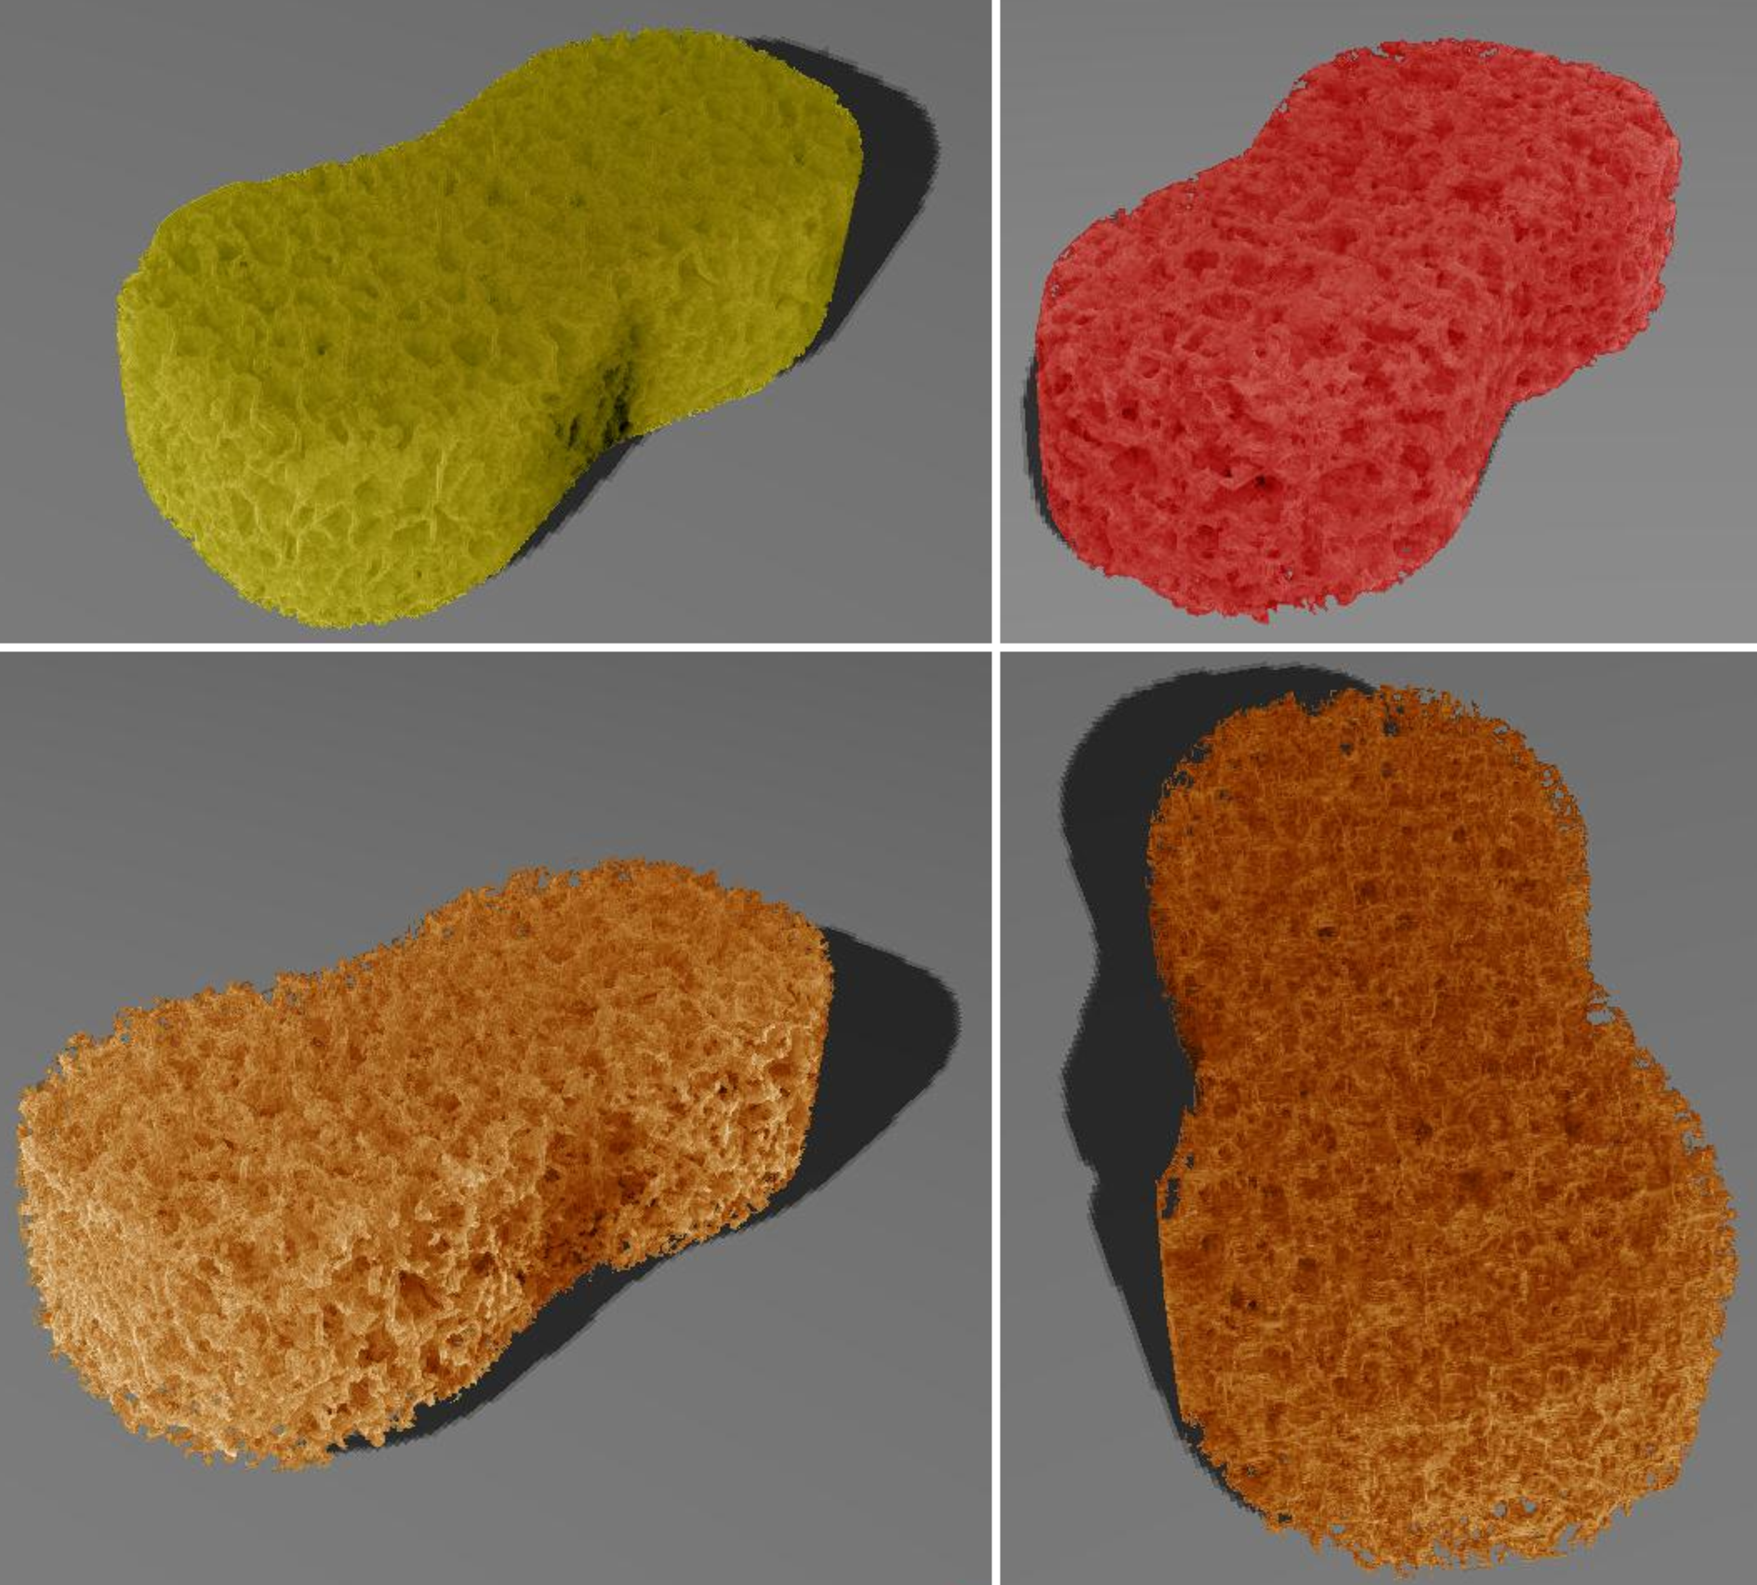
\includegraphics[width=7cm]{../figures/Fig13CAVW}}
\end{frame}

\begin{frame}{Piedras}

\centerline{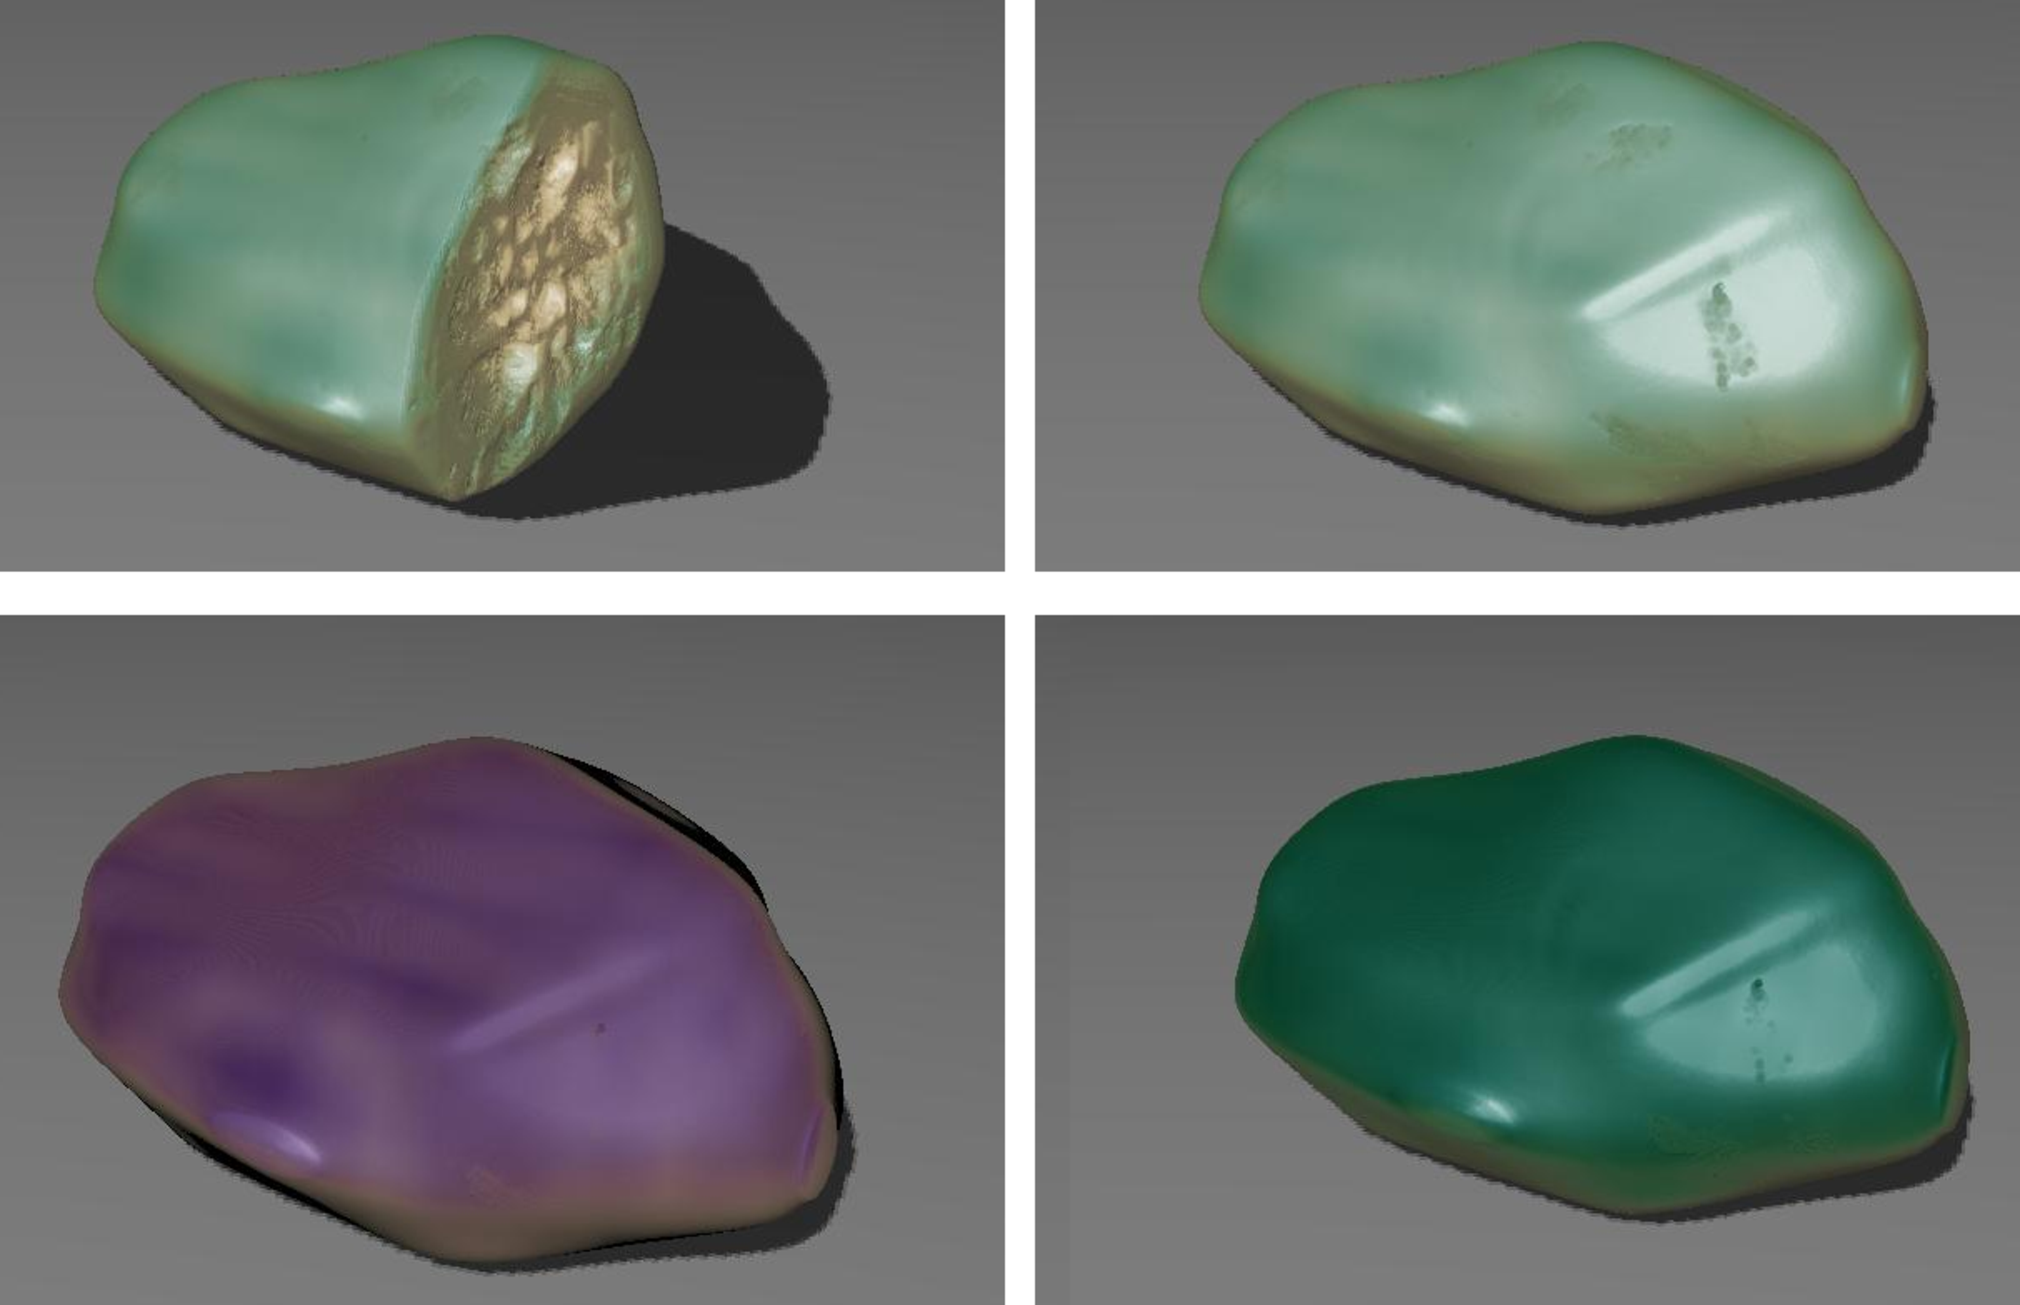
\includegraphics[width=9cm]{../figures/Fig14CAVW}}
\end{frame}

\subsection{Modelado procedimental de pan inspirado en su proceso de formación}
\begin{frame}
\begin{itemize}
\item Debido a que el proceso es extremadamente complejo, el mismo ha sido ignorado en gran medida en la literatura de computación gráfica.

\item Sin embargo, ha sido ampliamente estudiado en ingeniería de los alimentos.

\item No existe aún un modelo unificado. Los modelos existentes representan solamente subprocesos (cocción, leudado, formación de la corteza, etc.).

\item Es posible utilizar algunos de estos subprocesos para diseñar un algoritmo procedimental.
\end{itemize}
\end{frame}

\begin{frame}
\centerline{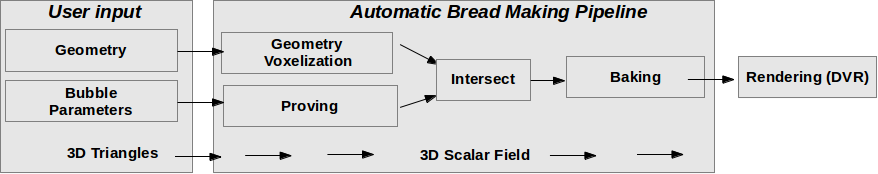
\includegraphics[width=12cm]{../figures/pipeline}}
\end{frame}

\begin{frame}{Leudado}
Se extraen esferas de un cubo, donde la cantidad de esferas $N(r)$ extraídas es inversamente proporcional al radio $r$ de la esfera, es decir, se utiliza la ley fractal

\begin{equation*}
N(r) = \frac{k}{r^{d}},
\end{equation*}

$k$ parámetro.

\centerline{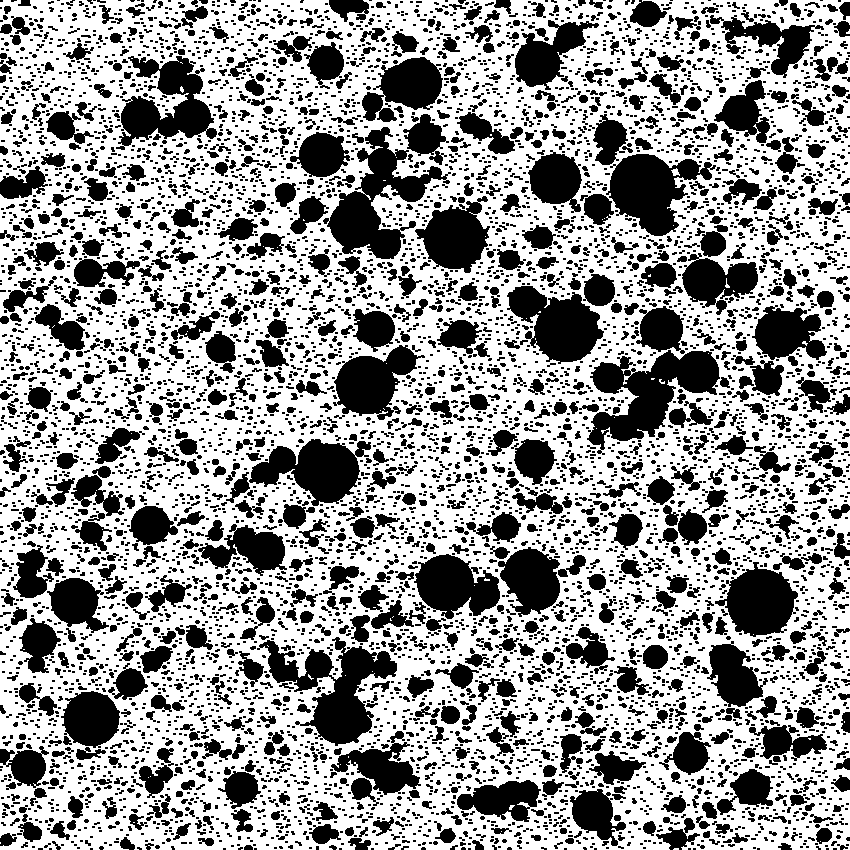
\includegraphics[width=6cm]{../figures/bubbles}}
\end{frame}

\begin{frame}
Si bien el proceso de generación utiliza una ley fractal, la intersección de las burbujas produce una estructura que no es necesariamente fractal, como se demostrará más adelante.

\vspace{1cm}

Es necesario disponer de las burbujas en una geometría de entrada, para esto, utilizar un enmascarado directo (multiplicación) produce resultados incorrectos:

\centerline{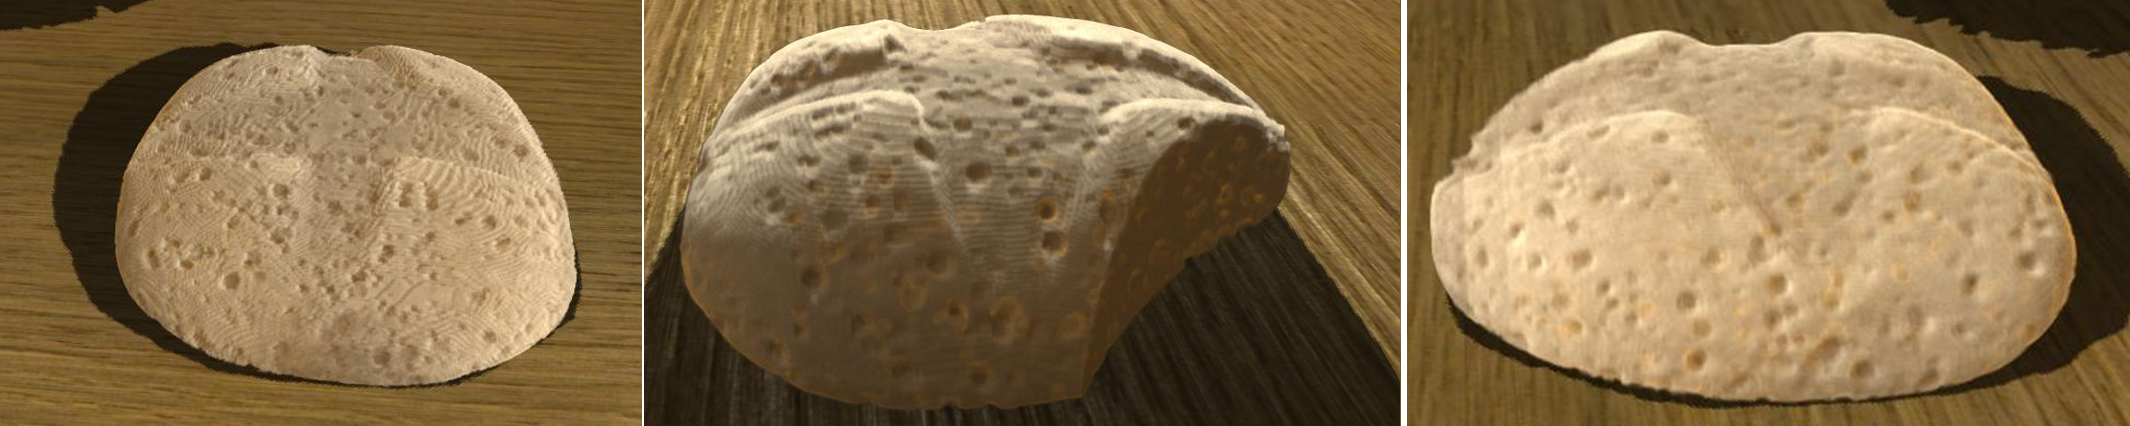
\includegraphics[width=8cm]{../figures/intersectProblem}}
\end{frame}

\begin{frame}
Se utiliza el mapa de distancias previamente discutido y un umbral, obteniéndose una región donde puede haber burbujas, permitiendo además obtener una corteza de ancho parametrizable.


\centerline{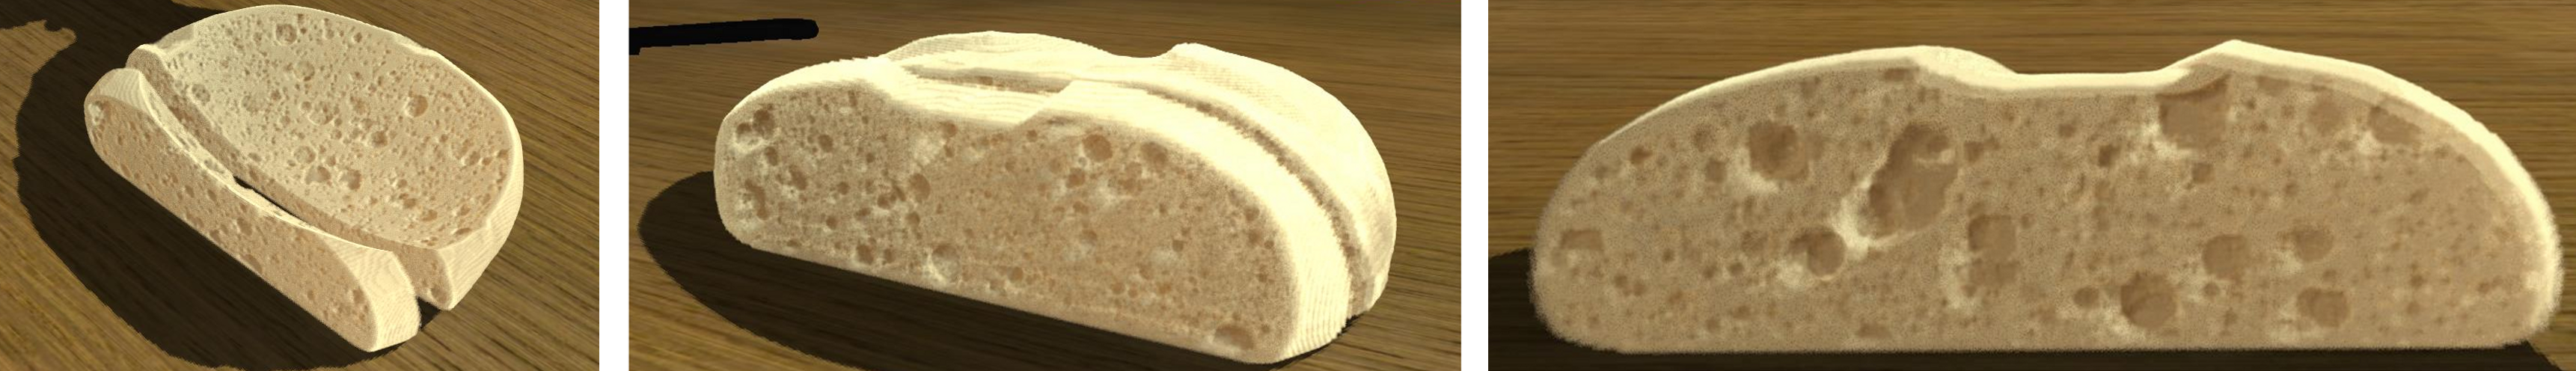
\includegraphics[width=10cm]{../figures/prebakebread}}
\centerline{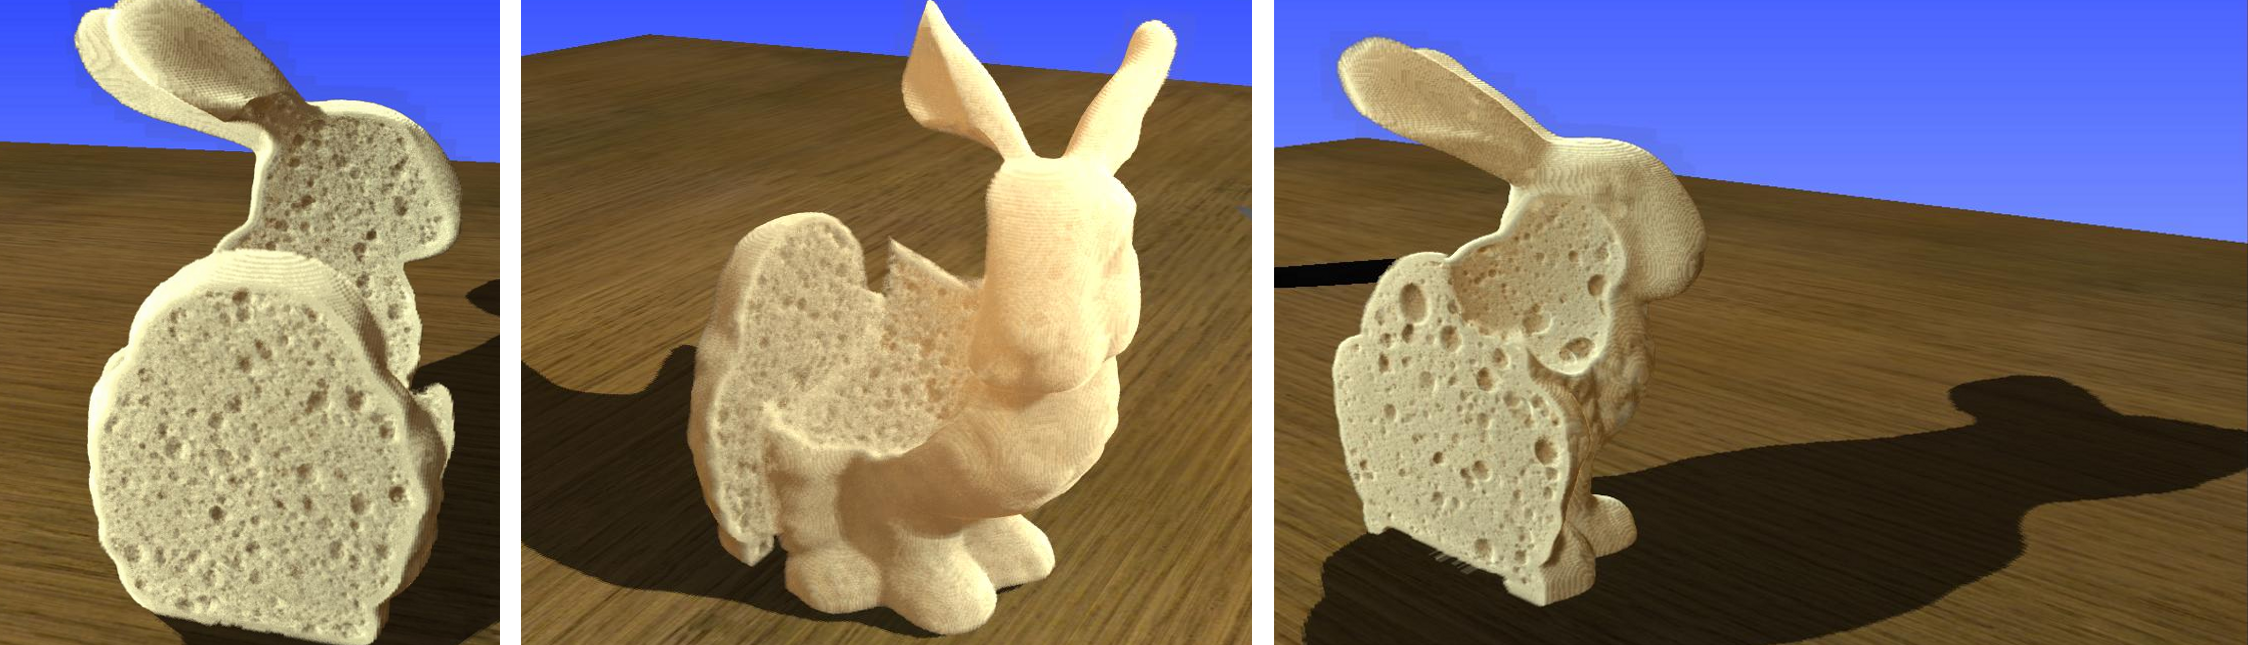
\includegraphics[width=10cm]{../figures/prebakebunny}}
\end{frame}


\begin{frame}{Cocción}
Procesos durante la cocción:

\begin{itemize}
\item Transferencia de calor y masa
\item Crecimiento de las burbujas
\item Deformación de la masa original
\item Formación de la corteza
\item Reacciones químicas
\end{itemize}

En nuestro caso, debe atenderse especialmente al efecto de dichos procesos sobre la \textbf{apariencia}.

\end{frame}

\begin{frame}{Cocción}
Modelo unidimensional

\begin{equation}
\label{Eq:heat}
\frac{\partial T}{\partial t} = \frac{1}{\rho C_{p}} \frac{\partial}{\partial x} \left ( k \frac{\partial T}{\partial x} \right ) + \frac{\lambda}{C_{p}} \frac{\partial W}{\partial t}+\frac{\lambda W}{ \rho C_{p} }\frac{\partial \rho}{\partial t},
\end{equation}
%
\noindent donde

$T$ temperatura, $x$ es la coordenada radial, $t$ tiempo, $C_{p}$ calor específico, $\rho$ densidad, $k$ conductividad térmica, $\lambda$ calor latente de la evaporación de agua, y $W(x,t)$ contenido de agua líquida.

Condiciones iniciales:
\begin{align*}
T(x,0) &= T_{0}(x), 0\le x \le L/2,
\end{align*}

\end{frame}

\begin{frame}{Cocción}
Condiciones de borde (continuidad y suavidad)
\begin{align*}
\left ( \frac{\partial T}{\partial x} \right )_{x=L/2} &= 0 , t > 0 \\
-k \left ( \frac{\partial T}{\partial x} \right )_{x=0} &= h_{r}(T_{r}-T_{s}) + h_{c}(T_{air}-T_{s}) - \lambda \rho D_{w} \left (\frac{\partial W}{\partial x} \right )_{x=0}
\end{align*}
%

\end{frame}

\begin{frame}
Horno a una temperatura típica (por defecto utilizamos $210^{\circ}C$) y discretiza el tiempo en intervalos $\Delta t = 30s$.


De la simulación se obtiene un arreglo unidimensional $Temp$, de tamaño $N_{grid}$, compuesto por valores de temperatura.

Luego, obtenemos una distribución 3D de la temperatura
\begin{equation*}
\displaystyle R_{vol}[x,y,z] = Temp[ round( DF_{M}[x,y,z] ) ], 
\end{equation*}

$DF_{M}[(x,y,z)] = 0 \rightarrow$ contorno, $Temp[0] \rightarrow R_{vol}[(x,y,z)]$.
$DF_{M}[(x,y,z)] > 0 \rightarrow$ interior, $<$ T  $\rightarrow R_{vol}[(x,y,z)]$, .

\centerline{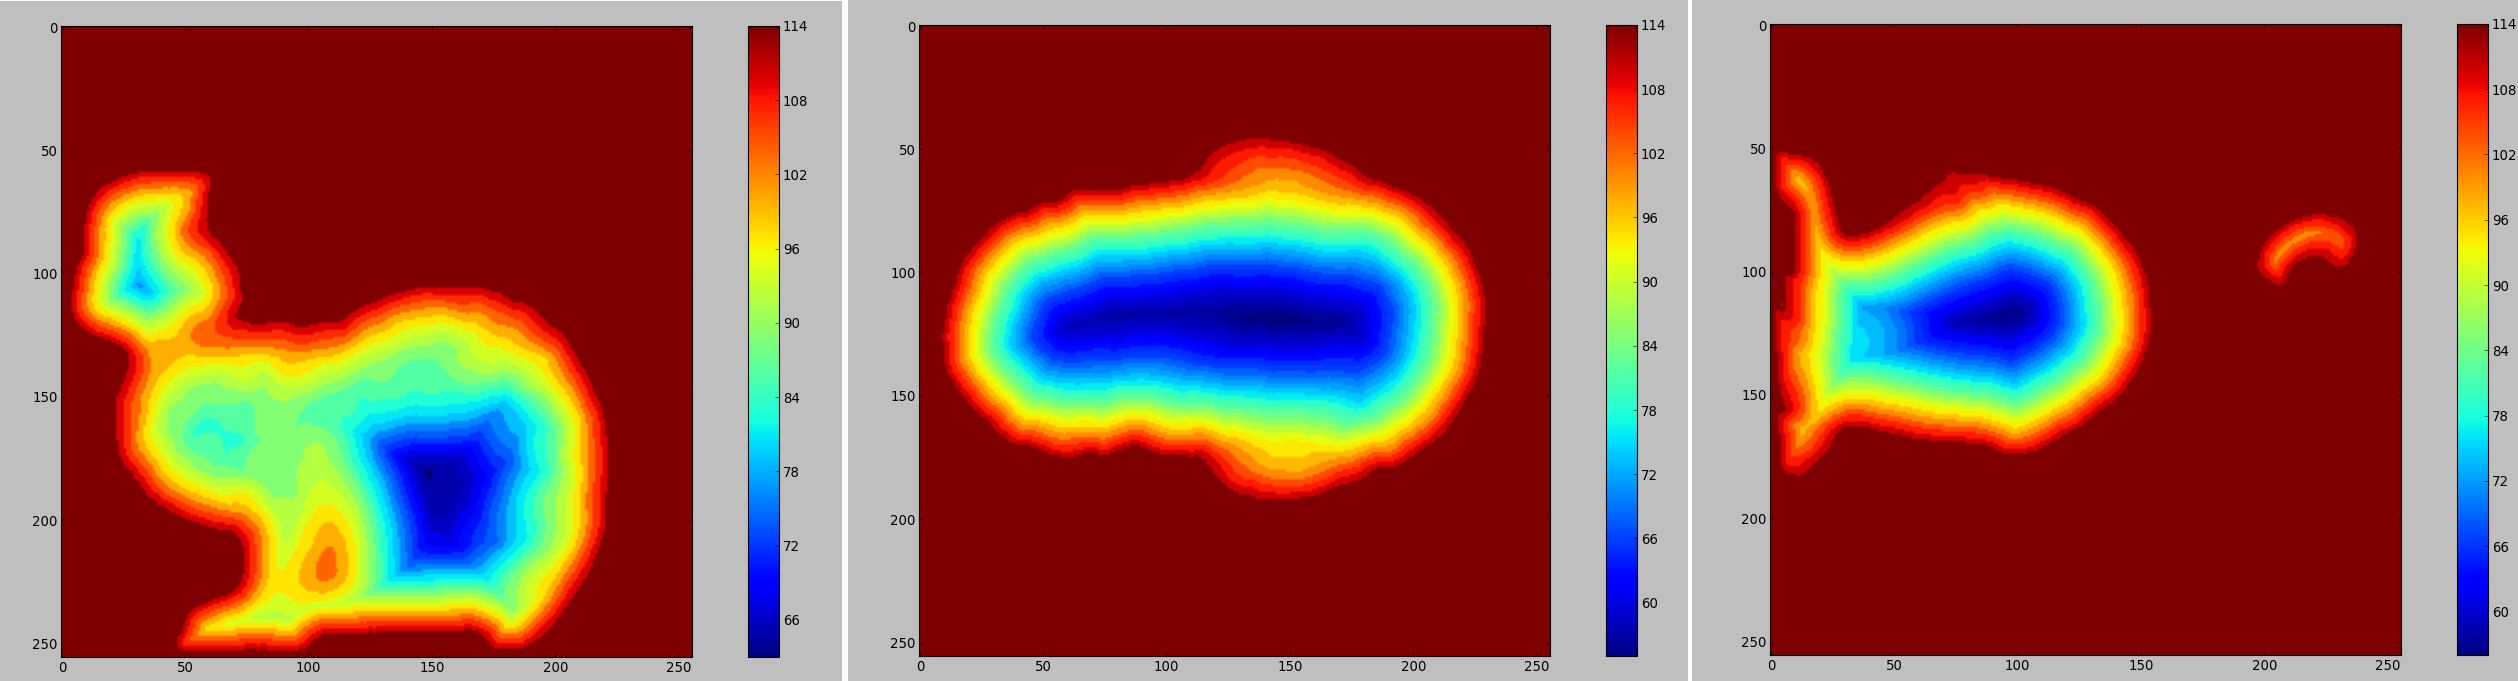
\includegraphics[width=8cm]{../figures/tempsbunny}}
\end{frame}

\begin{frame}{Deformación por Temperatura}

Utilizamos una operación de warping, deformando las burbujas de acuerdo a la temperatura, en tres dimensiones, reemplazando así los sistemas dinámicos de la sección anterior.

Se aplica un filtrado gaussiano al gradiente de $R_{vol}$, obteniendo $g'$

\begin{align*}
\displaystyle
[x,y,z] = [u,v,w] + p\, g'[u,v,w],
\end{align*}

Efecto de $p = 5,10,15$, respectivamente
\centerline{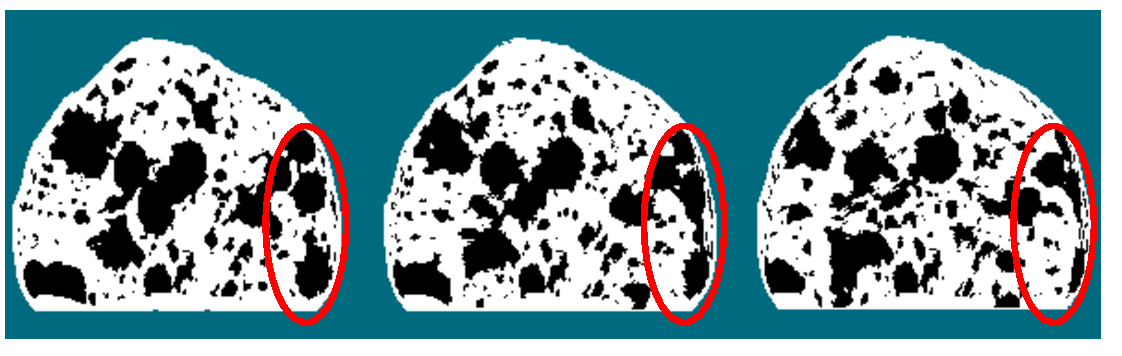
\includegraphics[width=12cm]{../figures/parameterp}}

\end{frame}

\begin{frame}{Levantamiento de la masa}

Una segunda operación simula el levantamiento de la masa, basado en la distribución de burbujas durante el leudado.
\begin{equation*}
P[x,y,z] = max \bigg\{r\bigg\}
\end{equation*}

El parámetro $p$ se trata localmente, entonces $p = P[u,v,w],$

\begin{equation*}
[r,s,t] = [u,v,w] + P[u,v,w] \, g'[u,v,w],
\end{equation*}

%\noindent donde $[u,v,w]$ es la entrada original, y $[r,s,t]$ es la coordenada deformada.


Finalmente, se escala la textura de acuerdo a la distribución de burbujas,


\begin{equation}
[x,y,z] = [r,s,t]\, S \, P[r,s,t],
\end{equation}

\noindent donde $[x,y,z]$ es la entrada final, luego de la deformación inducida por el crecimiento.

\end{frame}

\begin{frame}{Resultados}

\centerline{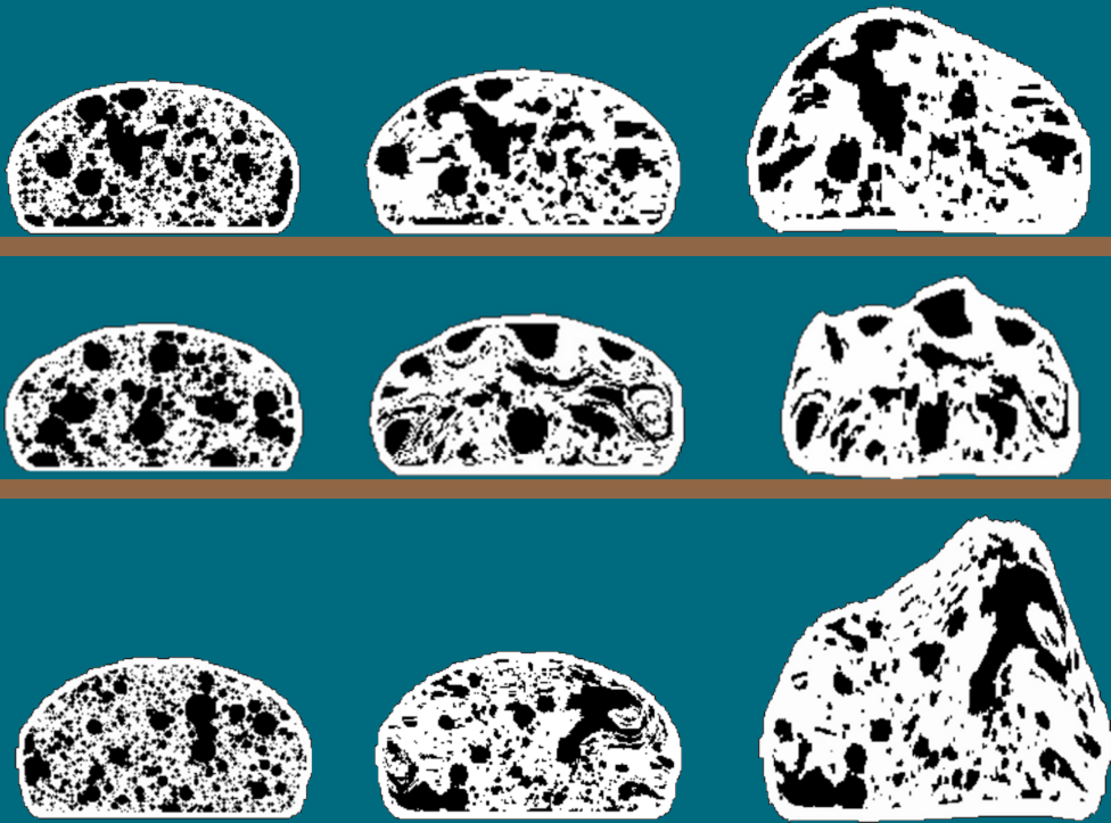
\includegraphics[width=9cm]{../figures/Fig9}}

\end{frame}

\begin{frame}{Corteza}
Tomamos colores CIELab de muestras reales, reportadas por Purlis et. al. (2009).

$$L = 40 \rightarrow \text{quemado}$$

$$L = 90 \rightarrow \text{crudo}$$

los canales $a$ y $b$ no están reportados, pero se obtuvieron de fotografías. Se observa que varian suavemente.

Estos colores se distribuyen de acuerdo a la distribución de masa en la corteza. Donde hay menor masa, el canal $L$ será menor y viceversa.

Se define la {\em densidad de la corteza} en cada posición de la textura volumétrica como $N_{v} / W_{size},$ donde $N_{v}$ es el número de voxels con valor $1$ en una ventana en el entorno de la posición, y $W_{size}$ es el número de voxels en esa ventana
\end{frame}



\begin{frame}{Resultados}

\centerline{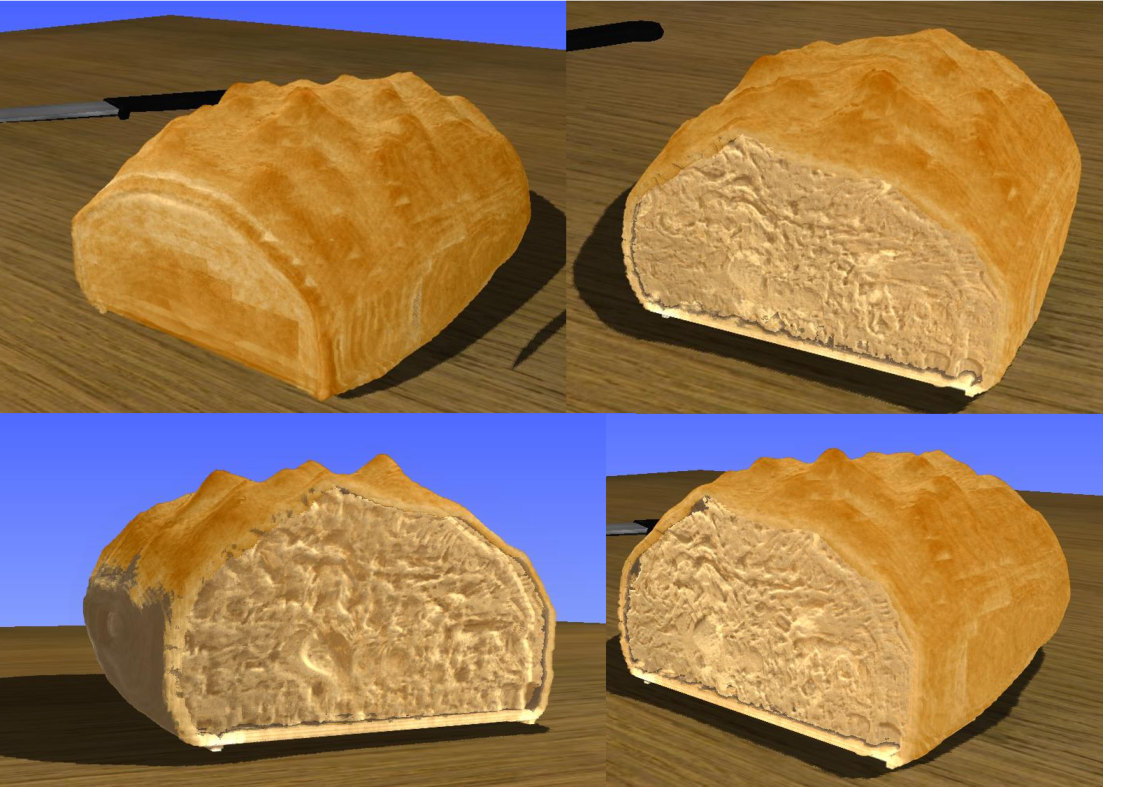
\includegraphics[width=9cm]{../figures/Fig11}}

$S$ con valores aleatorios en cada punto, picos visibles en la corteza.

\end{frame}

\begin{frame}{Resultados}

\centerline{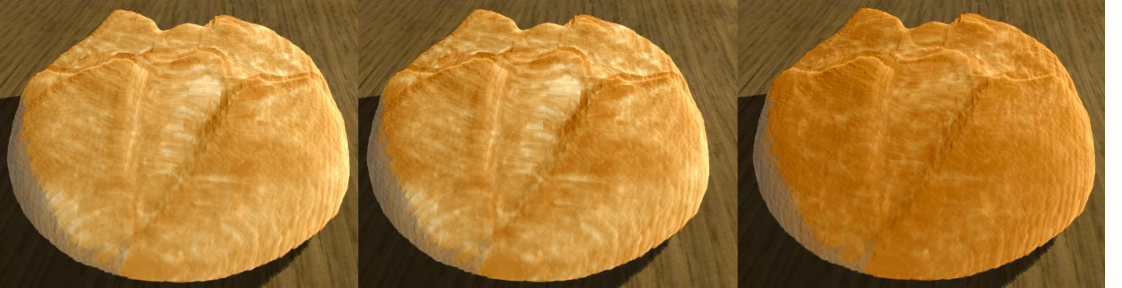
\includegraphics[width=12cm]{../figures/Fig13}}
Cortezas con diferentes historias de cocción. De izquierda a derecha, se decrementa el valor máximo admitido para el canal $L$.

\end{frame}

\begin{frame}{Resultados}
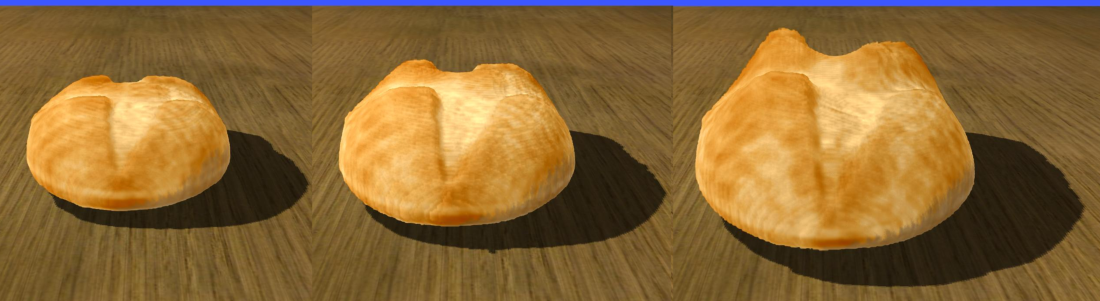
\includegraphics[width=11cm]{../figures/Fig14}

Panes luego de la cocción mostrando diferentes crecimientos. De izquierda a derecha se incrementa el parámetro $S$.

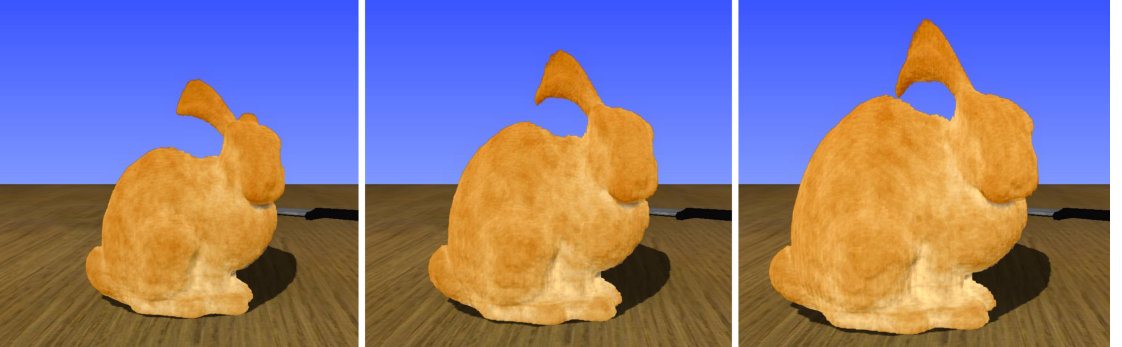
\includegraphics[width=9cm]{../figures/Fig15}


\end{frame}

\begin{frame}{Tiempos de Cómputo}

\begin{table}[h!]
       % Give a unique label
% For LaTeX tables use
\begin{tabular}{lllll}
\hline\noalign{\smallskip}
Resolución de la Textura Volumétrica & $256^{3}$ & $384^{3}$  & $512^{3}$ \\
\noalign{\smallskip}\hline\noalign{\smallskip}
Leudado & 3.62 & 12.07 & 31.29 \\
Intersección & 8 & 10.27 & 14.97 \\
Transformación de Distancia & 7 & 23.73 & 56 \\
Cocción  & 49.81 & 144.69 & 313.7 \\
\hline\noalign{\smallskip}
Total & 68.43 & 190.76 & 415.96 \\
%Rendering & 1s & 4s & 0\% \\
\noalign{\smallskip}\hline
\end{tabular}
\caption{Tiempos de cómputo típicos en de las distintas etapas de la fabricación sintética de pan, expresados en segundos.}
\label{tab:computingtimes}
\end{table}
\end{frame}

\begin{frame}{Conclusiones}
\begin{block}{}
\begin{itemize}
\item Modelo inspirado físicamente
\item Elimina decisiones ad-hoc
\item Se simula cocción, levantamiento de la masa, etc.
\item Permite obtener imágenes en sucesivas etapas del proceso de formación
\end{itemize}
\end{block}
\end{frame}

\section{Renderización}

\begin{frame}{Renderización}

Muchas técnicas de renderizado utilizan mallas para computar los resultados.

En nuestro caso, contamos con una textura volumétrica, por lo tanto proponemos utilizar Renderizado Directo de Volúmenes para evitar la construcción de una malla.

Además, de esta forma será posible obtener cortes arbitrarios del material.

\end{frame}

\begin{frame}{DVR}
DVR aproxima la Ecuación del Transporte Radiativo (RTE).

Se computa un \textbf{rayo} para cada pixel, desde la pantalla al objeto. El algoritmo computa el cambio de radiancia a lo largo del medio.


\centerline{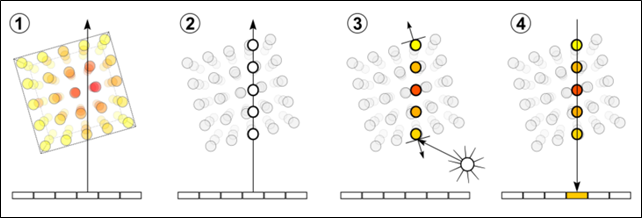
\includegraphics[width=9cm]{../figures/dvr}}

Para obtener resultados en tiempo real, tomamos una versión simplificada de la RTE, teniendo en cuenta sólamente la transmitancia.
\end{frame}

\begin{frame}{Renderización}


Sea el coeficiente de absorción $ = \int_{p_i}^{p_j} k_a(t) \, dt$  $ = \tau_{(p_i, p_j)}$.


Entonces la Transmitancia es la cantidad de luz que \texttt{atraviesa} un segmento del volumen:

\begin{equation*}
  T(p_i,p_j) = e^{-\tau_{(p_i, p_j)}}.
\end{equation*}

Radiancia: cantidad de luz que pasa o es emitida por un medio.

\begin{equation*}
  L(p_n) = L_b \ e^{-\tau(p_0, p_n)} + \int_{p_0}^{p_n} \rho \ e^{-\tau(t,p_n)} \, dt.
\end{equation*}

(Radiancia de fondo $+$ Radiancia del medio) \\

La implementación reemplazará la integral por una suma,

\begin{equation*}
  L(p_n) = L_b \ e^{-\tau(p_0, p_n)} + \sum_{p_0}^{p_n} \rho \ e^{-\tau(p_i,p_n)}.
\end{equation*}


\end{frame}


\begin{frame}{DVR en GPU}
\centering
En el fragment shader,
\begin{itemize}
\item Computamos un rayo principal desde la cámara hacia el volumen
\item Además, en cada paso del rayo, un rayo secundario computa la transmitancia desde la posición actual hacia la luz, produciendo sombras naturales
\end{itemize}


\centerline{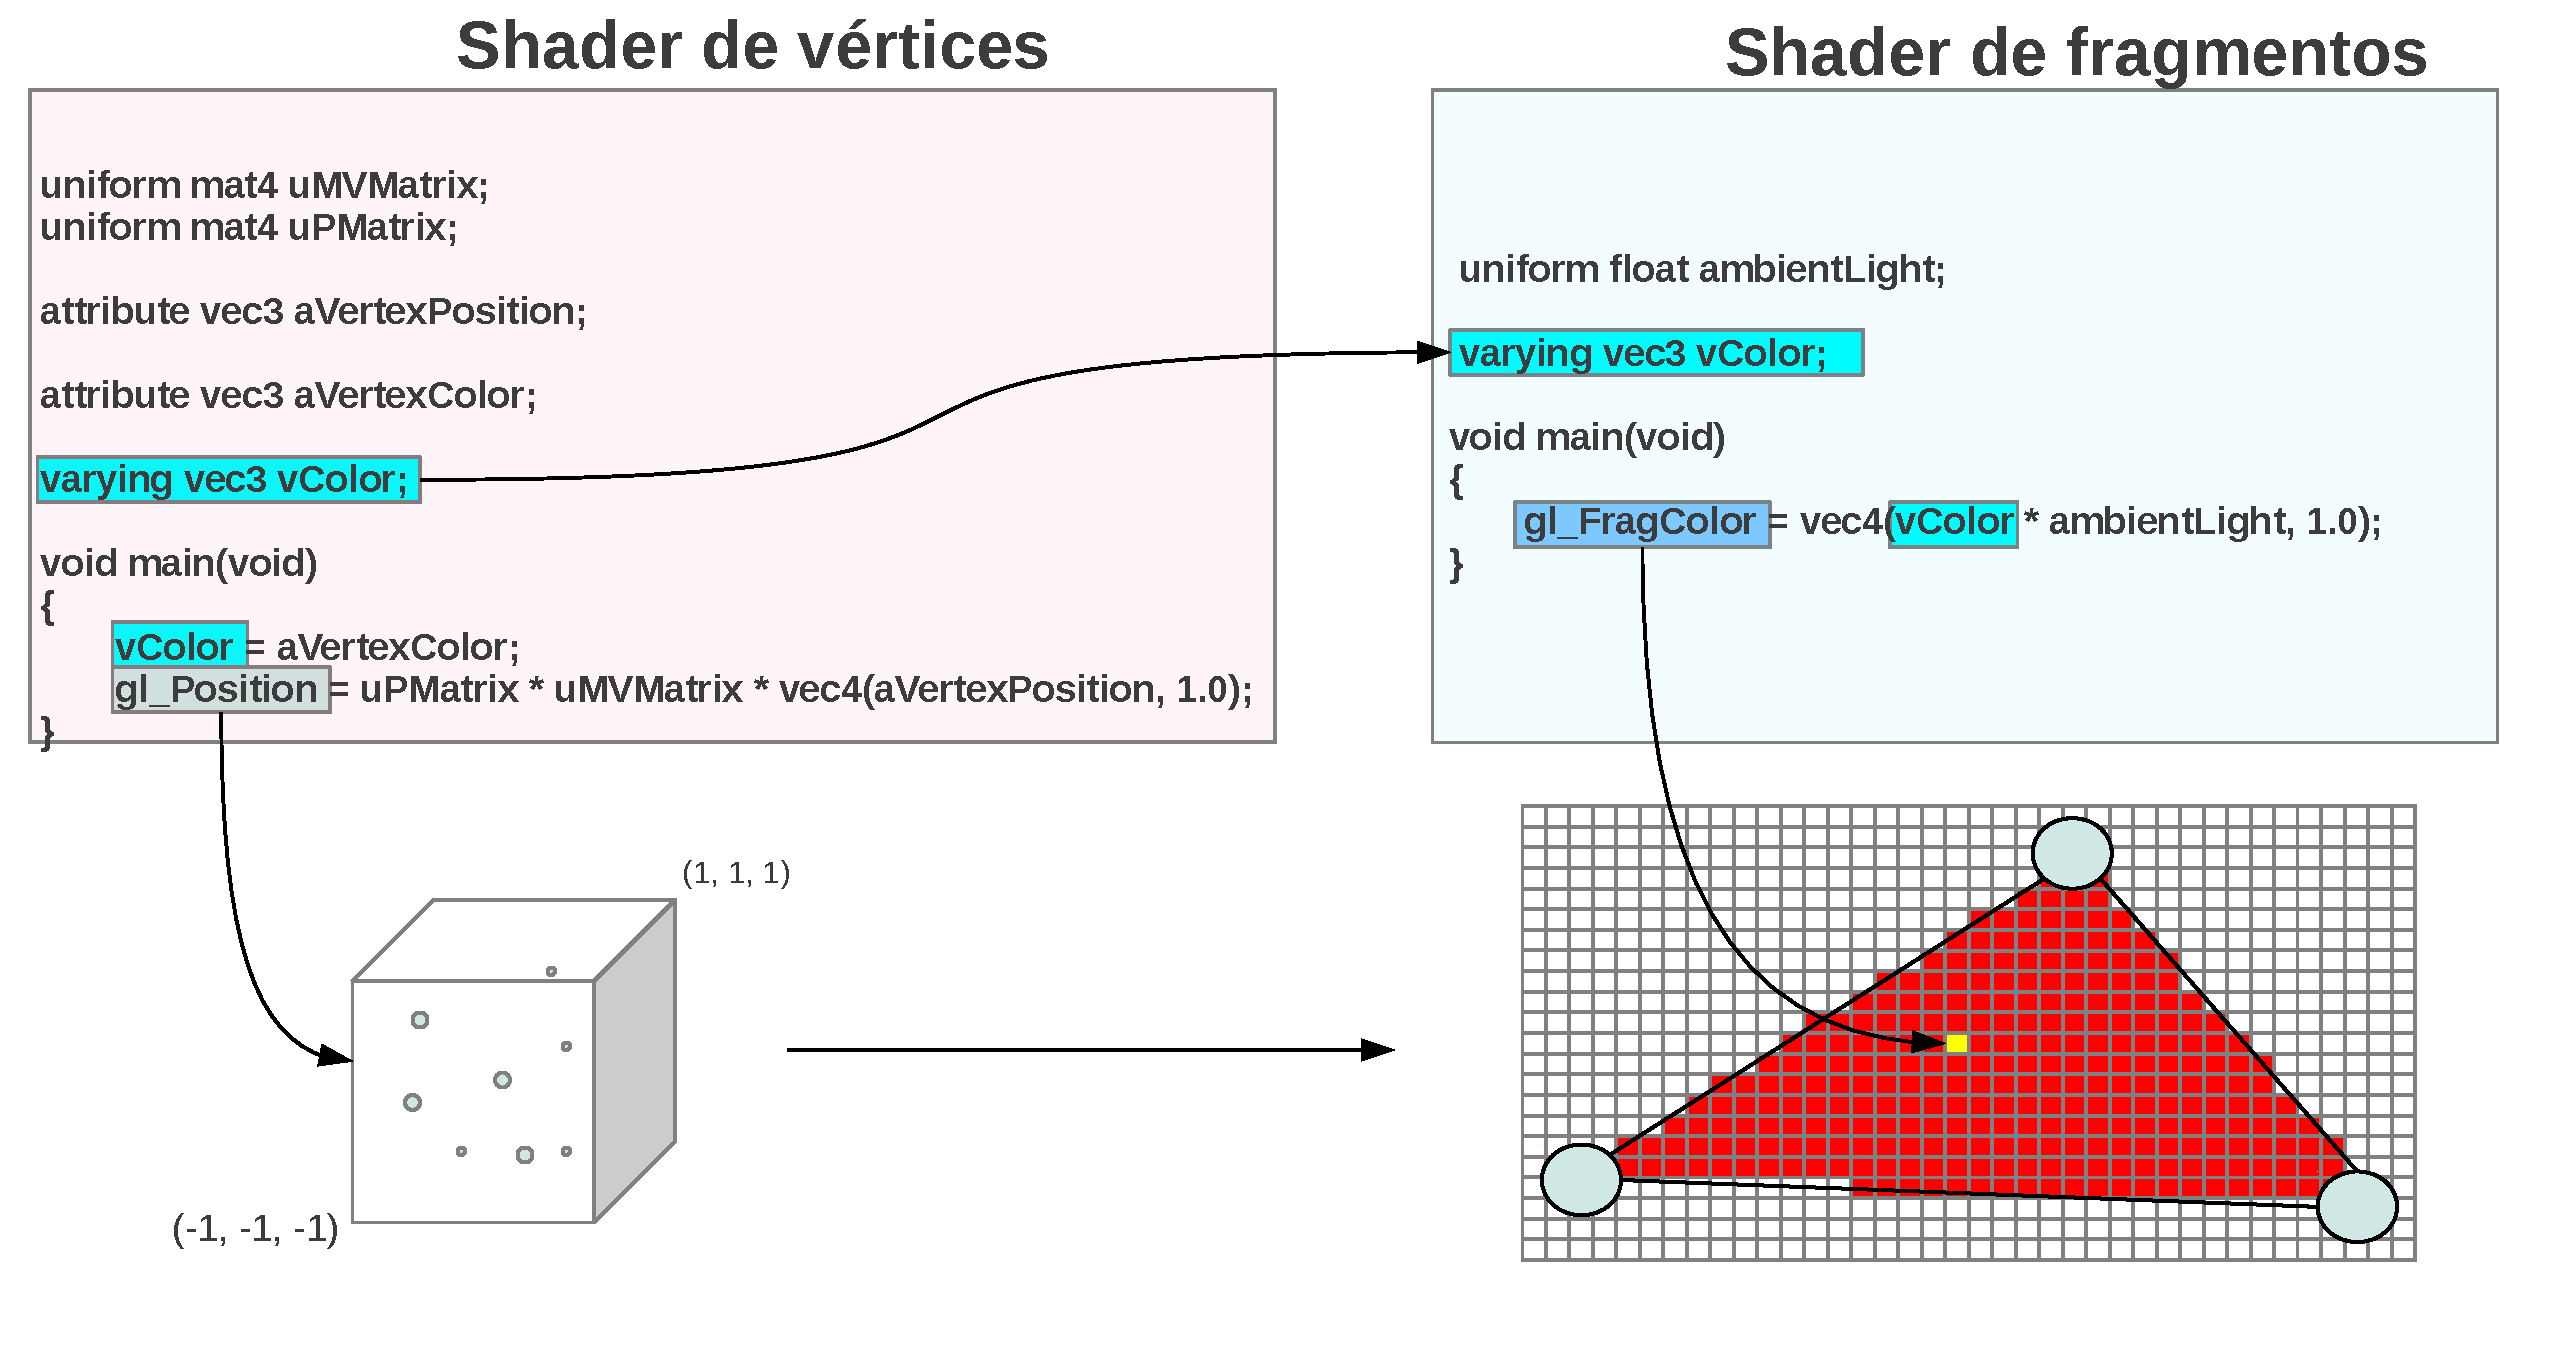
\includegraphics[width=4cm]{../figures/fragmentshader}}


\end{frame}

\begin{frame}{Tiempos de Cómputo}

\begin{table}[htb]
\centering
%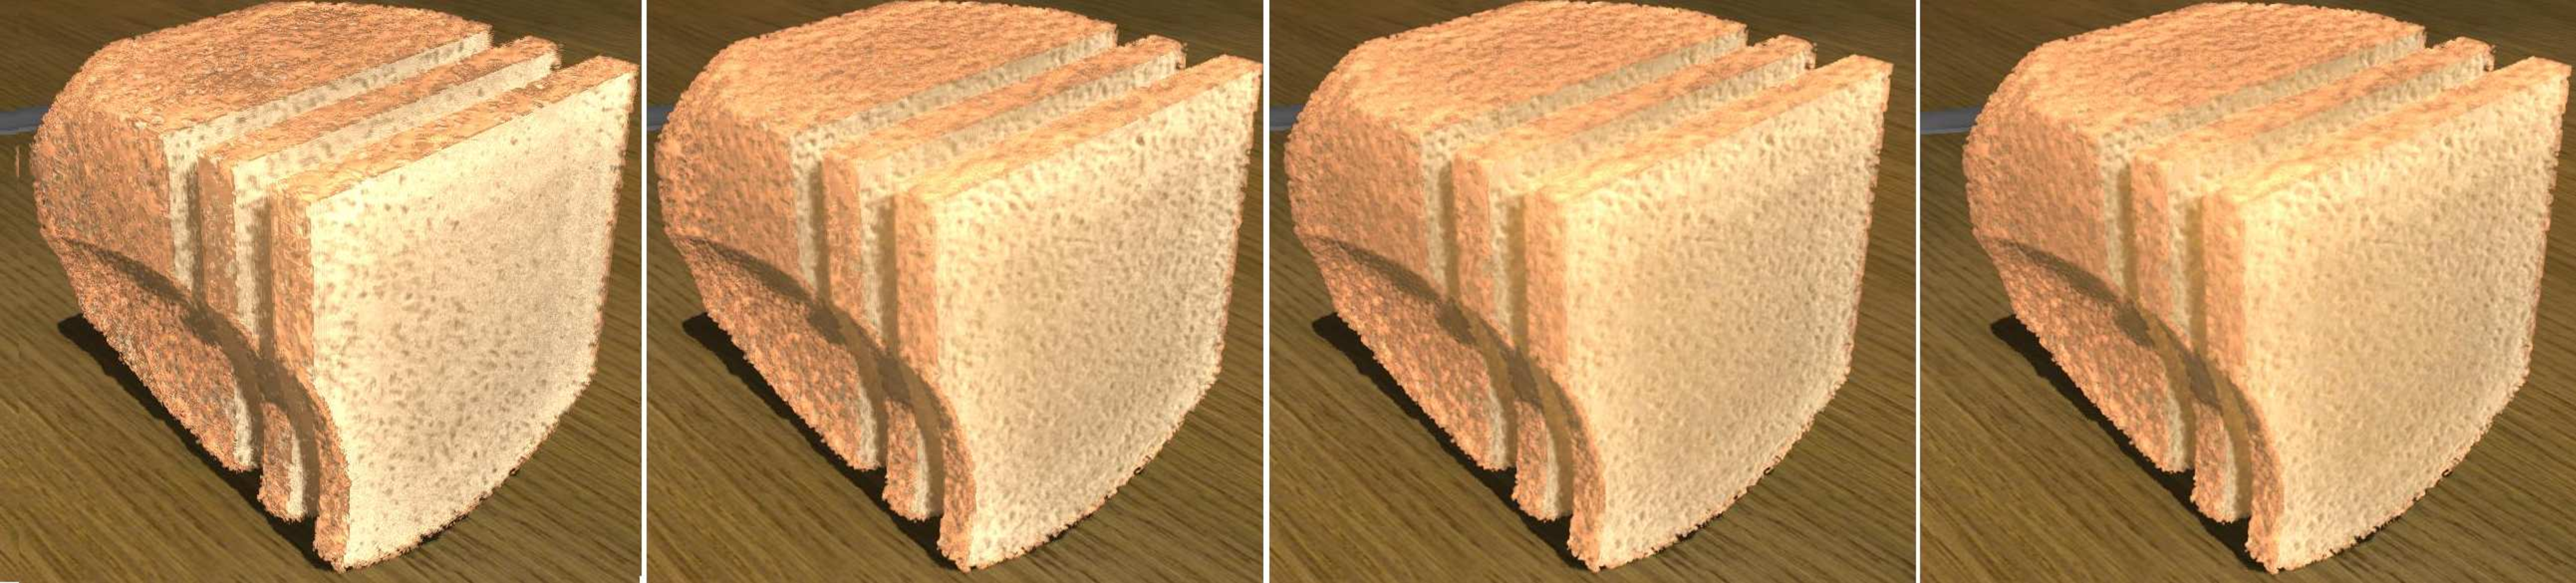
\includegraphics[width=12cm]{stepcount.pdf}

\begin{tabular}{|c|c|c|c|c|c|c|}
\hline
 Pasos del rayo         & 128 &  256 \\
\hline
\hline
 Tiempo total shaders   & 10 ms &  32.5 ms \\
\hline
 Rayo Principal         & 2 ms  & 5 ms  \\
\hline
 Rayos Secundarios      &  8 ms & 27.5 ms  \\
\hline
\end{tabular}
\caption{Detalle de tiempos de renderizado en milisegundos.}
\label{tab:n2}
\end{table}


\end{frame}

\begin{frame}{Renderizado con más de una escala}
A la hora de obtener complejidad en la imagen resultante, existen limitaciones en la resolución de la textura.

Una solución consiste en utilizar más de una textura

\centerline{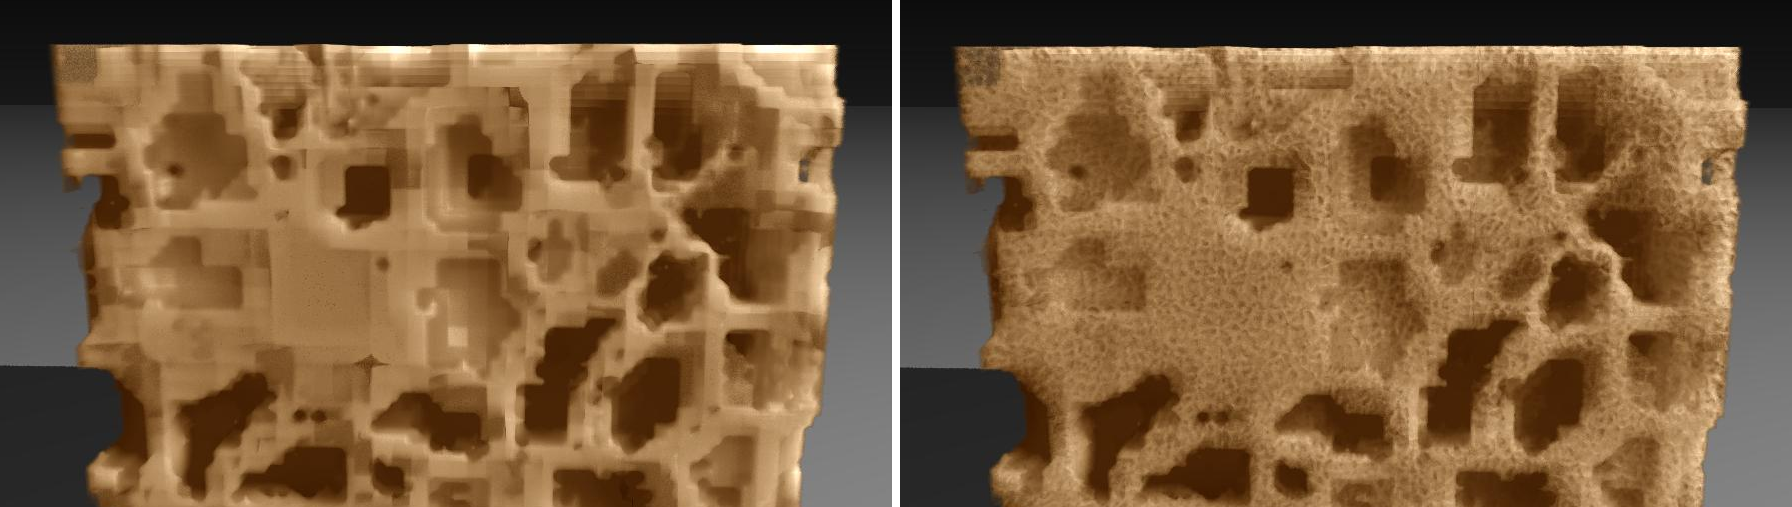
\includegraphics[width=10cm]{../figures/multiscale}}

Textura A muestreada en $(x,y,z)$

Textura B muestreada en $N\times (x,y,z), N \in \mathbb{R}$

\end{frame}



\begin{frame}{Conclusiones}
\begin{itemize}
\item Imágenes realistas
\item Tiempo real
\item Implementación simple
\end{itemize}

\begin{block}{Trabajos a Futuro}
\begin{itemize}
\item Otros materiales
\end{itemize}
\end{block}
\end{frame}

\section{Validación}

\begin{frame}{Espectro Multifractal}

\end{frame}

\subsection{Extras}

\begin{frame}{Clasificación de Imágenes de cortes de Pan}

\end{frame}

\begin{frame}{Validación utilizando Aprendizaje Profundo}
Recientemente se desarrollaron técnicas de Aprendizaje Profundo, los cuales clasifican una imagen entre miles de clases.

Los clasificadores se encuentran online, por lo cual es sencillo probar la clasificación con las imágenes generadas. Los resultados en panes son promisorios

\centerline{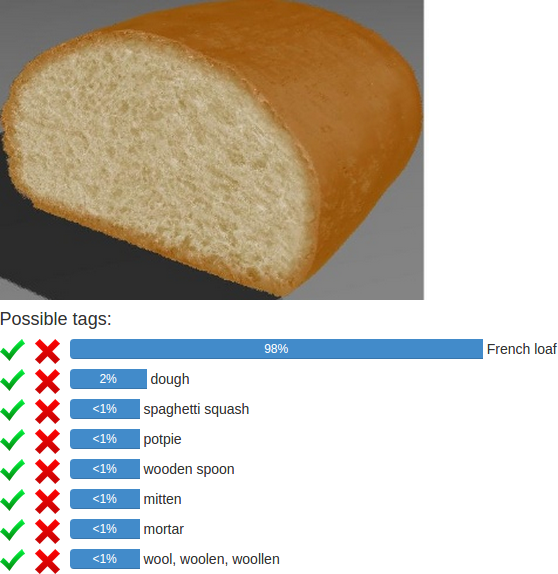
\includegraphics[width=5cm]{../figures/deep1}}

\end{frame}

\begin{frame}{Validación utilizando Aprendizaje Profundo}

\centerline{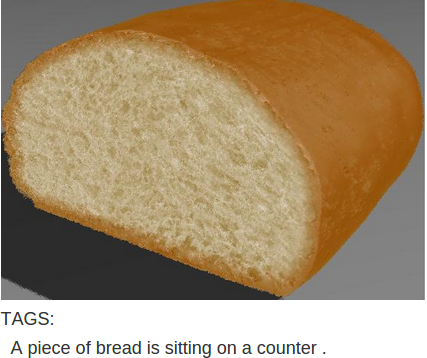
\includegraphics[width=4cm]{../figures/deep2}}
\centerline{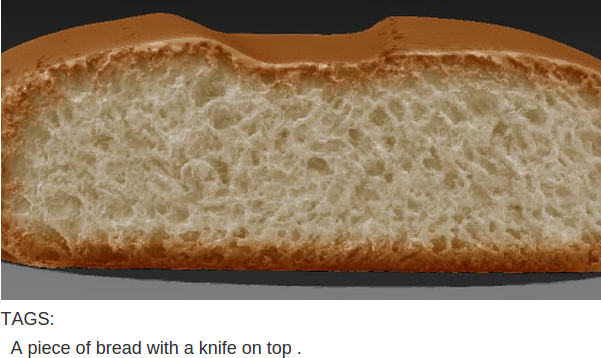
\includegraphics[width=4cm]{../figures/deep3}}
\end{frame}
\begin{frame}{Validación utilizando Aprendizaje Profundo}
\centerline{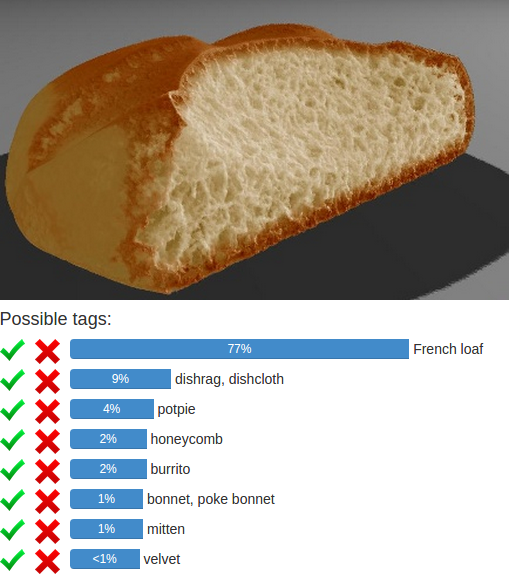
\includegraphics[width=5cm]{../figures/deep4}}

\end{frame}


\section{Conclusiones y Trabajos a Futuro}

\begin{frame}
\centering

?`Preguntas?

\end{frame}

\begin{frame}
\centering

!`Gracias!

\end{frame}
\end{document}
